\documentclass[12pt,a4paper]{article}

%% ── Packages ────────────────────────────────────────────────────────────────
\usepackage[margin=2.5cm]{geometry}
\usepackage{amsmath,amssymb}
\usepackage{booktabs}
\usepackage{graphicx}
\usepackage{subcaption}
\usepackage{hyperref}
\usepackage{xcolor}
\usepackage{listings}
\usepackage{float}
\usepackage{enumitem}
\usepackage{multirow}
\usepackage{array}
\usepackage{parskip}
\usepackage{titlesec}
\usepackage{fancyhdr}
\usepackage{caption}
\usepackage[expansion=false]{microtype}

\hypersetup{colorlinks=true, linkcolor=blue!70!black, citecolor=blue!70!black, urlcolor=blue}

\lstset{
  basicstyle=\ttfamily\small,
  breaklines=true,
  frame=single,
  backgroundcolor=\color{gray!8},
  keywordstyle=\color{blue},
  commentstyle=\color{gray},
}

\setlength{\headheight}{14.5pt}
\pagestyle{fancy}
\fancyhf{}
\chead{\small ME228 --- Fatigue Strength Prediction \& Inverse Alloy Design}
\rfoot{\thepage}

%% ── Title ───────────────────────────────────────────────────────────────────
\title{
  \Large\textbf{ME228 --- Applied Data Science and Machine Learning}\\[2pt]
  \large\textit{Final Project Report}\\[6pt]
  \LARGE Data-Driven Fatigue Strength Prediction\\
         and Inverse Alloy Design for Low-Alloy Steels\\[8pt]
  \large Mixture-of-Experts Regression with Empirical Reliability and\\
         Cost-Constrained Pareto Recommendation
}
\author{
  Nishit Dharamshi (24b2153) \quad Shourya Saxena (24b2222) \\[2pt]
  Kapidhwaj Soni (24b2214) \quad Rudra Khandelwal (24b2140)
}
\date{April 2026}

\begin{document}
\maketitle
\tableofcontents
\newpage

% ─────────────────────────────────────────────────────────────────────────────
\section{Executive Summary}
% ─────────────────────────────────────────────────────────────────────────────

Fatigue accounts for 80--90\,\% of mechanical structural failures~\cite{agrawal2014}, yet
rotating-bending fatigue tests are destructive, slow ($>$10\textsuperscript{7} cycles per
specimen), and expensive. We present a complete \emph{forward + inverse} machine-learning
pipeline that, for low-alloy steels:

\begin{enumerate}[nosep]
  \item Predicts rotating-bending fatigue strength (10\textsuperscript{7} cycles, MPa) from
        chemical composition and heat-treatment parameters using a two-expert ensemble.
  \item Reports a calibrated Probability of Failure (PoF) under a user-specified applied
        stress, validated against out-of-fold (OOF) residual distribution rather than a naive
        Gaussian assumption.
  \item Inversely designs the cheapest viable alloy + heat-treatment recipe given a target
        Factor of Safety, using neighbourhood sampling, kNN data-hull filtering, and Pareto
        analysis over (cost, PoF) objectives.
\end{enumerate}

\paragraph{Headline numbers.}
On the NIMS Fatigue Strength Dataset ($N\,{=}\,437$, 26 features):
\begin{itemize}[nosep]
  \item Non-carburised regime ($N\,{=}\,389$): 5-fold CV RMSE = $19.91 \pm 2.55$\,MPa.
  \item Carburised regime ($N\,{=}\,48$): 5-fold CV RMSE = $40.42 \pm 14.62$\,MPa.
  \item Held-out 20\,\% test: NC $R^2 = 0.97$, C $R^2 = 0.85$.
  \item Three of four canonical AISI grades (4140 QT, 4340 QT, 8620 carburised) predicted
        within handbook range; AISI 1045 (plain-carbon) over-predicted, defining the
        applicability boundary.
\end{itemize}


% ─────────────────────────────────────────────────────────────────────────────
\section{Problem Statement}
% ─────────────────────────────────────────────────────────────────────────────

\subsection{Engineering Context}
A materials engineer choosing an alloy for a fatigue-loaded component (shaft, gear, spring)
must answer two coupled questions:
\begin{enumerate}[nosep]
  \item \emph{Forward}: \textit{Will this alloy + heat-treatment survive the design load?}
  \item \emph{Inverse}: \textit{What is the cheapest alloy that meets the design load
        with a given safety margin?}
\end{enumerate}
Empirical S--N curves answer (1) only for catalogued grades; question (2) requires either
exhaustive testing or a predictive model that can interpolate the composition $\times$
heat-treatment space.

\subsection{Dataset}
We use the public NIMS MatNavi Fatigue Dataset~\cite{agrawal2014}: 437 experimental records
of rotating-bending fatigue strength (10\textsuperscript{7} cycles) for low-alloy steels.
Each record carries 26 input features and one target (Fatigue, MPa):
\begin{itemize}[nosep]
  \item \textbf{Chemical composition} (9 vars): C, Si, Mn, P, S, Ni, Cr, Cu, Mo (wt\,\%).
  \item \textbf{Heat-treatment} (13 vars): normalising (NT), through-hardening (THT, THt,
        THQCr), carburising (CT, Ct), diffusion (DT, Dt), quenching (QmT), tempering (TT,
        Tt, TCr).
  \item \textbf{Mill / specimen} (4 vars): reduction ratio (RedRatio), inclusion proxies
        (dA, dB, dC).
\end{itemize}

The target distribution is \emph{strongly bimodal}: carburised steels (CT\,=\,930\,°C,
$N\,{=}\,48$) cluster between 838 and 1190\,MPa, while non-carburised samples
($N\,{=}\,389$) span 225--906\,MPa with a right-skew. This bimodality directly motivates
the architectural choice in §\ref{sec:arch}.

\begin{figure}[H]
\centering
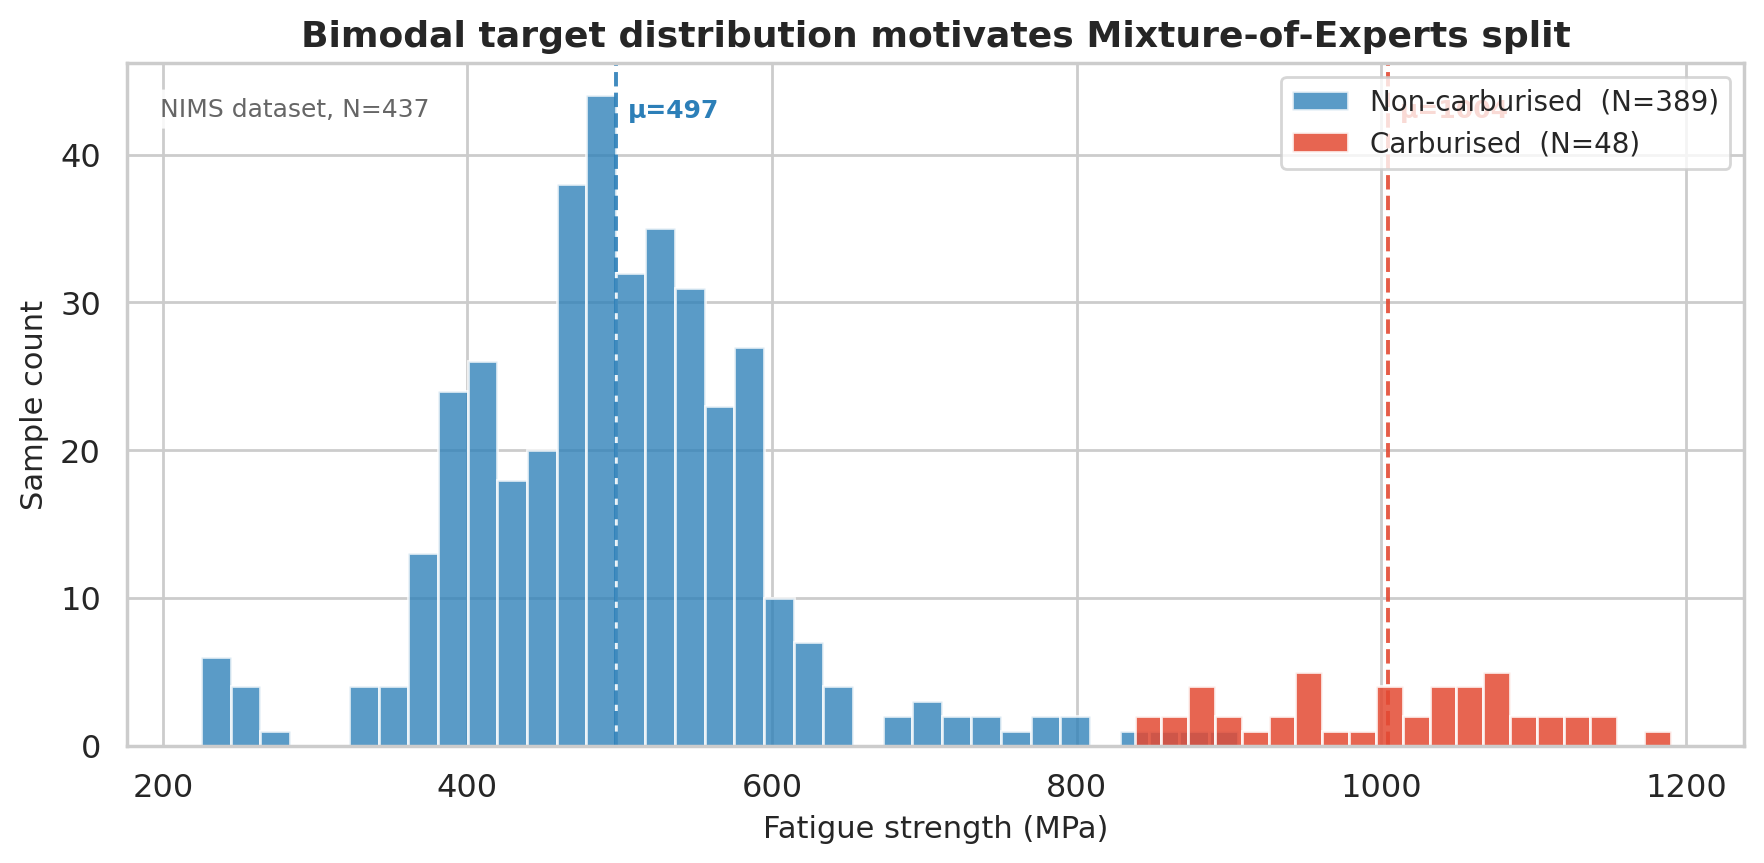
\includegraphics[width=0.92\textwidth]{slides_plots/01_bimodality.png}
\caption{Empirical fatigue-strength distribution for the NIMS dataset ($N=437$). The two
         modes correspond to physically distinct strengthening mechanisms: through-hardening
         (NC, blue, $\mu=497$\,MPa) and case-hardening via carburisation (C, red,
         $\mu\approx1007$\,MPa). The gap between modes is $>$250\,MPa, making a single
         global model inappropriate.}
\label{fig:bimodal}
\end{figure}

\subsection{Applicability Boundary}
The dataset is overwhelmingly populated by \emph{alloyed} low-alloy steels — non-zero Cr,
Mn, and frequently Mo or Ni. External validation (§\ref{sec:ext}) shows that predictions
on plain-carbon grades (e.g.\ AISI 1045 with Cr\,$<$\,0.1\,wt\%) are unreliable. We
explicitly restrict the deployed model to the alloyed regime
(Cr\,+\,Ni\,+\,Mo\,$\geq$\,0.1\,wt\%).


% ─────────────────────────────────────────────────────────────────────────────
\section{Final Architecture}\label{sec:arch}
% ─────────────────────────────────────────────────────────────────────────────

\begin{figure}[H]
\centering
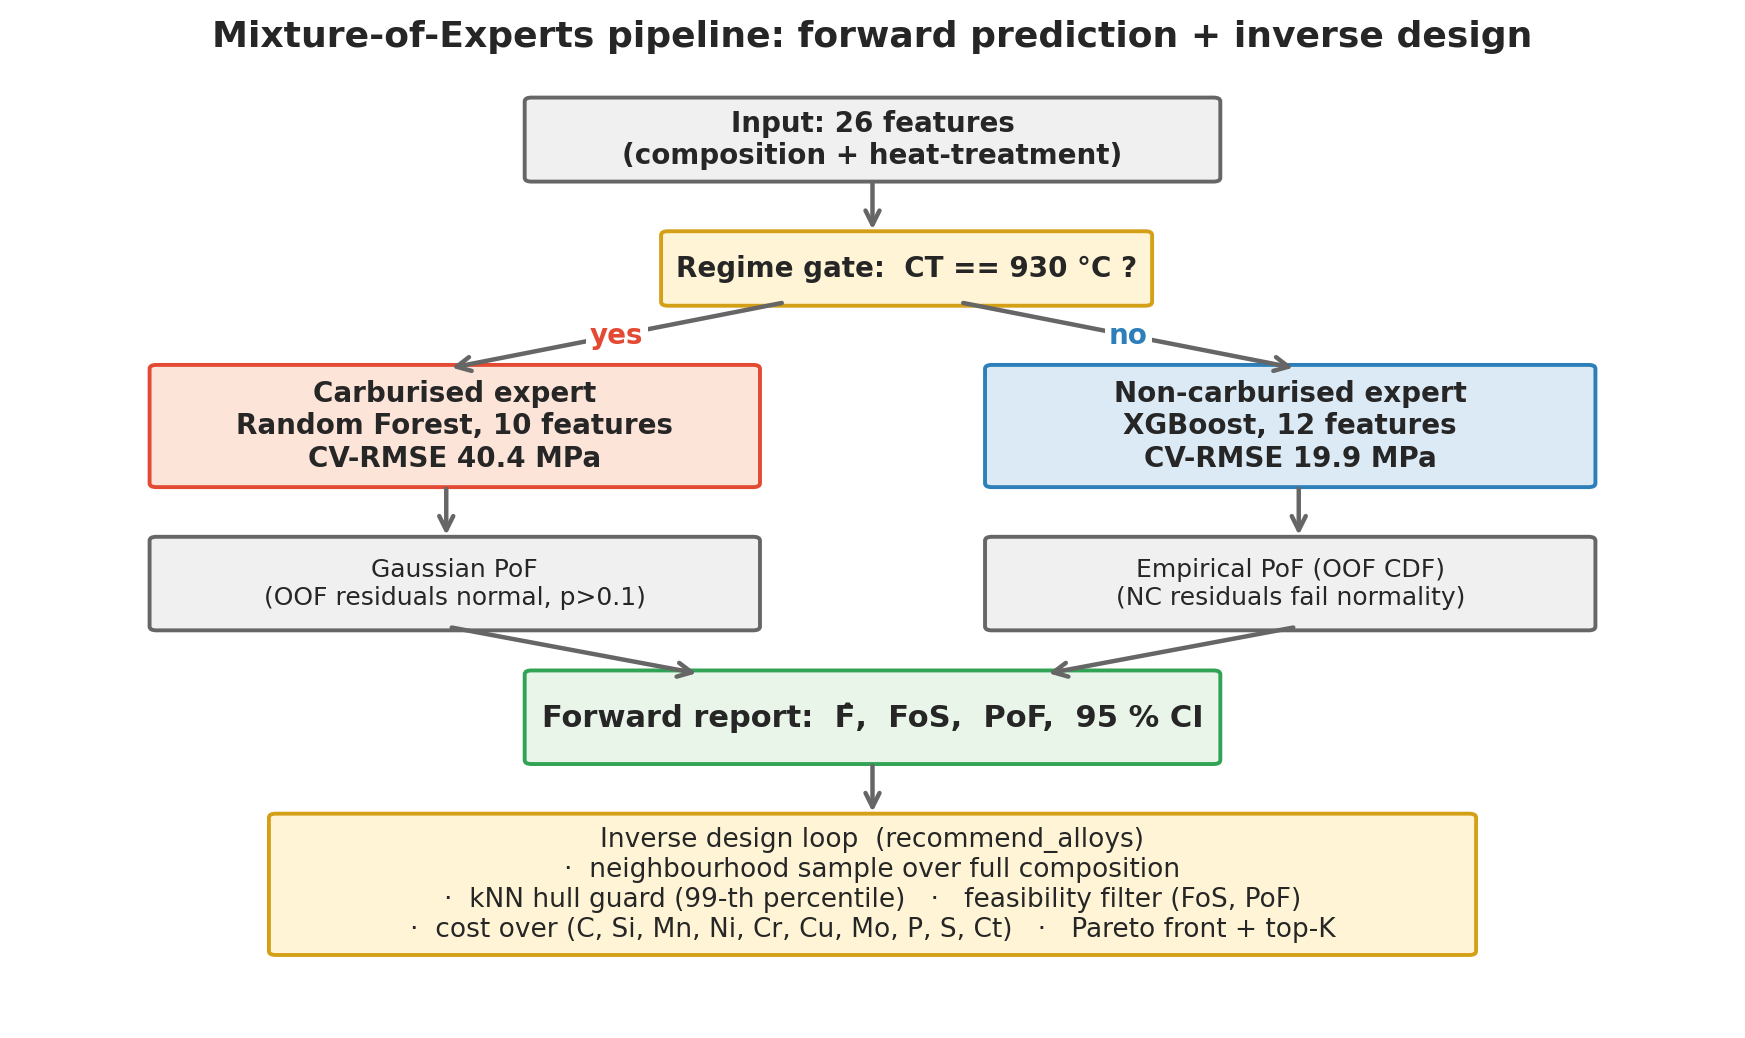
\includegraphics[width=0.85\textwidth]{slides_plots/02_architecture.png}
\caption{Final pipeline. A hard regime gate ($CT = 930\,^\circ$C) routes each input to the
         appropriate expert. The NC expert (XGBoost, 12 features, CV-RMSE 19.9\,MPa) uses
         an empirical OOF CDF for PoF; the C expert (Random Forest, 10 features, CV-RMSE
         40.4\,MPa) uses a Gaussian PoF. Both experts feed the same forward report and
         inverse design loop.}
\label{fig:arch}
\end{figure}

\subsection{Why Mixture-of-Experts (MoE)}\label{sec:moe}
A single global model averages two physically distinct strengthening mechanisms
(case-hardening vs.\ through-hardening) and produces an inflated, regime-blind error.
We engineer a binary gate
\[
  \texttt{is\_carburized} = \mathbf{1}[\,CT = 930\,]
\]
and route to two independent experts.

\textbf{Honest comparison.} A tuned global XGBoost achieves a pooled 5-fold CV RMSE of
23.1\,MPa, while the MoE pair achieves 23.1\,MPa pooled. The MoE does \emph{not} win on
pooled accuracy; it wins on \emph{regime-specific uncertainty}. The carburised regime has
its own residual distribution and its own physically grounded $\sigma$, which is essential
for trustworthy PoF reporting. MoE versus a linear baseline (Ridge / Lasso) gives the often-cited
$\sim$30\,\% RMSE reduction; against a tuned non-linear model the gain is in calibration, not
point error.

\subsection{Per-regime Model Choice}
A 5-fold CV bake-off across six families on regime features (defaults, no tuning):

\begin{table}[H]
\centering
\caption{Untuned 5-fold CV RMSE per regime. Bold = chosen family.}
\label{tab:bakeoff}
\begin{tabular}{lrr}
\toprule
\textbf{Model} & \textbf{NC RMSE (MPa)} & \textbf{C RMSE (MPa)} \\
\midrule
GP-Matern        & 20.36 ± 2.45 & 55.95 ± 17.71 \\
GBM (sklearn)    & 21.53 ± 2.62 & 53.82 ± 9.30 \\
\textbf{XGBoost} & \textbf{23.37 ± 2.67} & 57.74 ± 16.69 \\
\textbf{Random Forest} & 25.34 ± 1.81 & \textbf{45.83 ± 11.81} \\
Ridge            & 33.56 ± 1.27 & 53.09 ± 18.86 \\
kNN ($k=7$)      & 44.05 ± 1.13 & 65.20 ± 19.65 \\
\bottomrule
\end{tabular}
\end{table}

\textbf{NC (XGBoost).} Tuned XGBoost reaches 19.9\,MPa, beating GP-Matern (20.4\,MPa
untuned). XGBoost handles the right-skewed target without an explicit transform (we tested
$\log_1p(F)$; gain was 1.4\,\%, not worth complexity).

\textbf{C (Random Forest).} With $N\,{=}\,48$, RF's bagging and aggressive depth-limit make
it strictly more robust than XGBoost's boosting cascade. Tuned RF: 40.4\,MPa.

\begin{figure}[H]
\centering
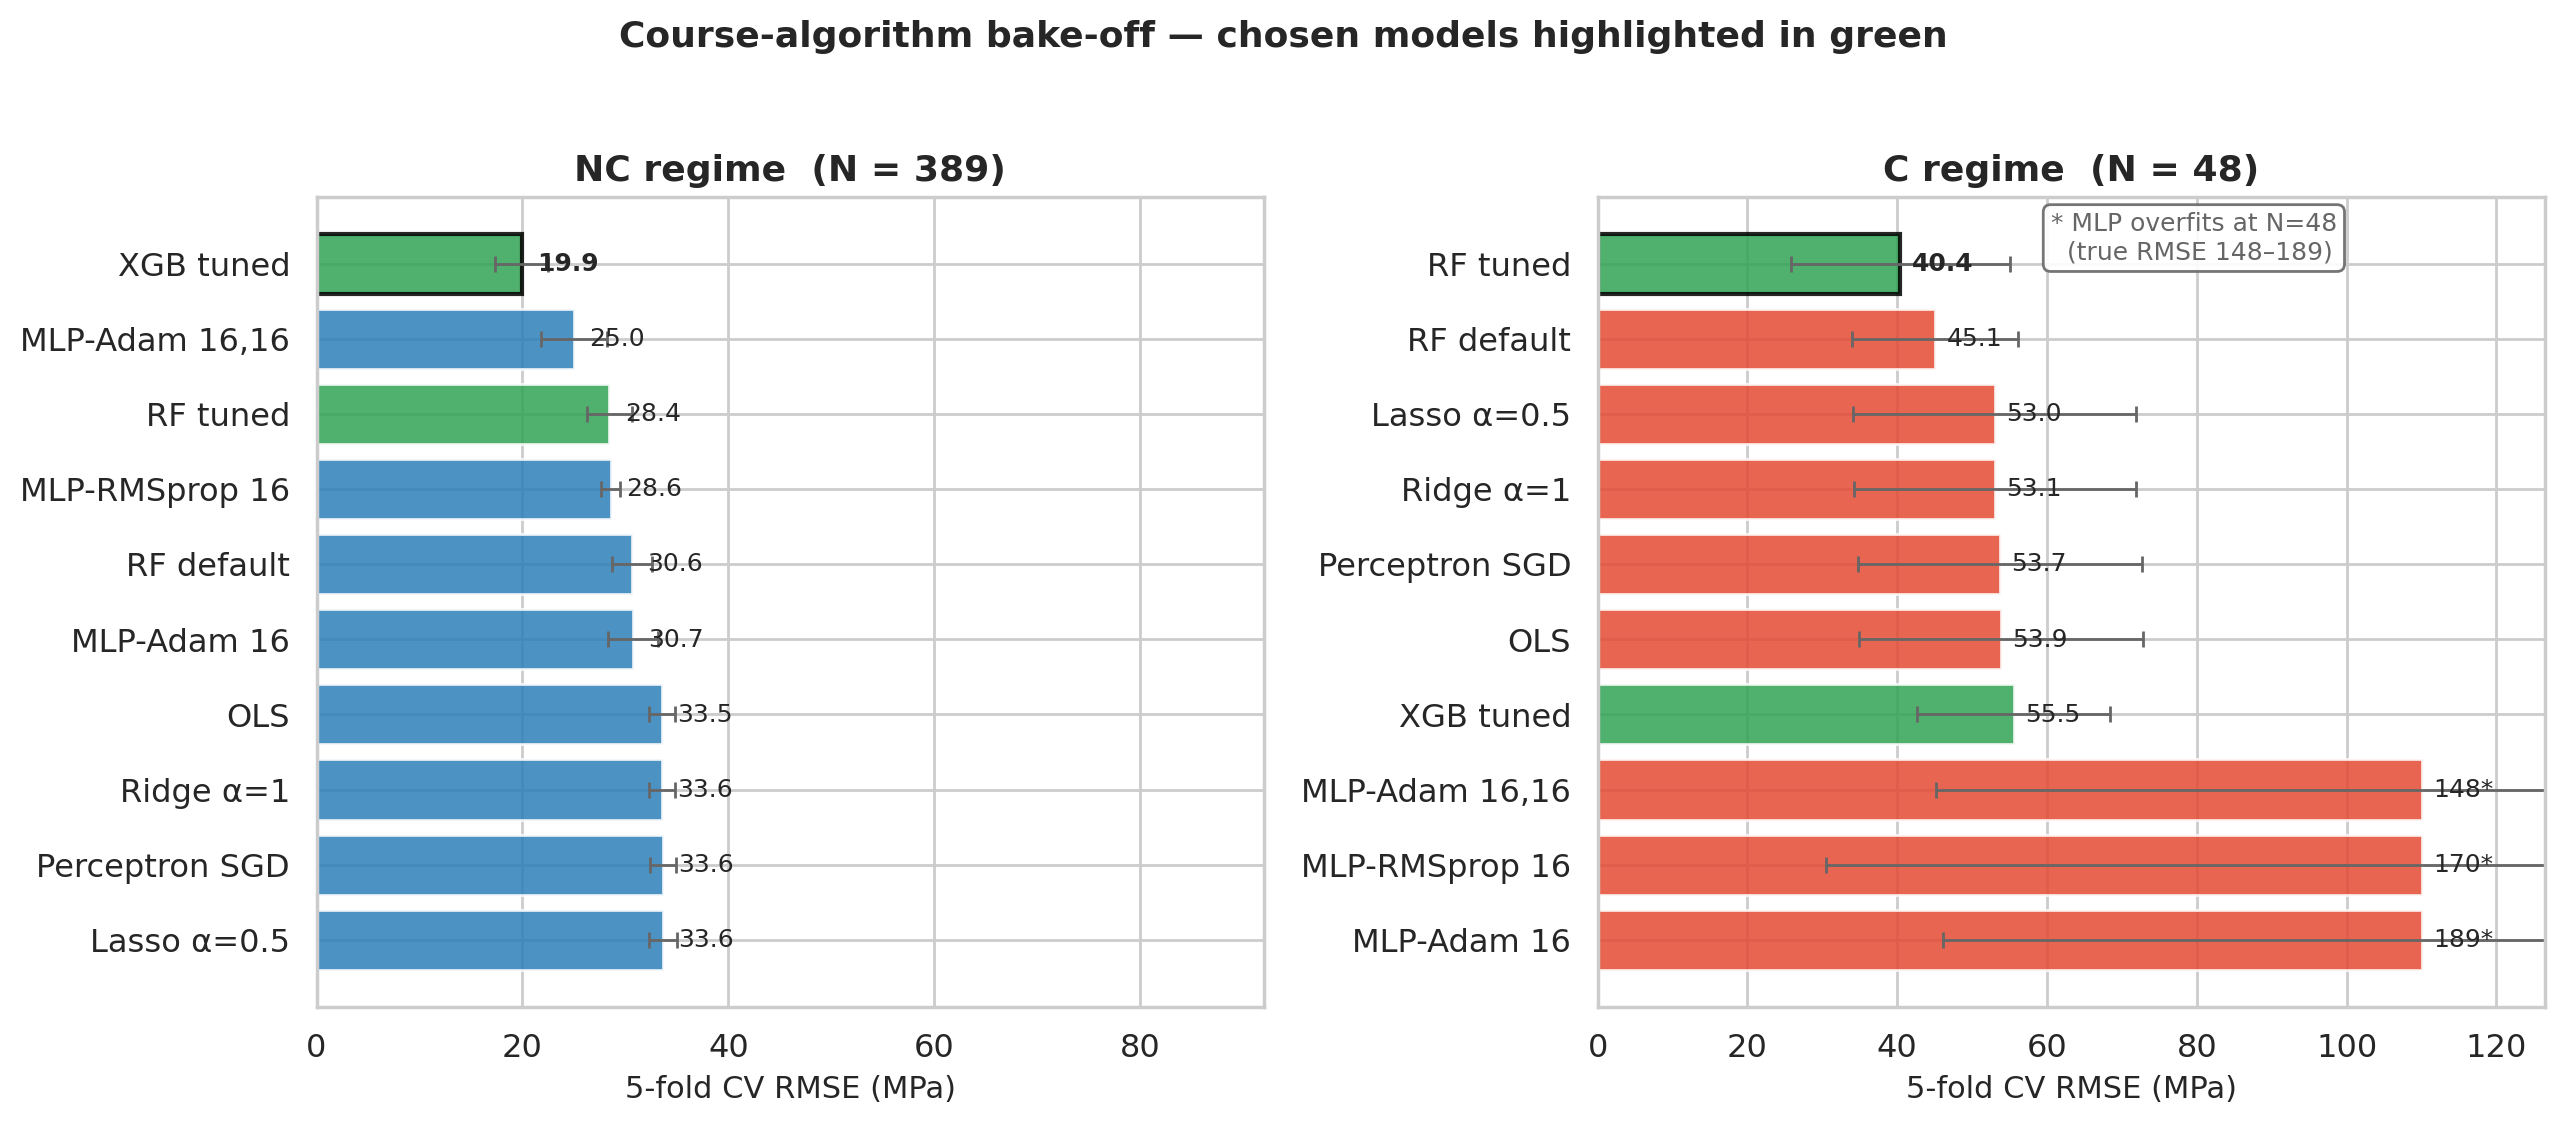
\includegraphics[width=\textwidth]{slides_plots/03_bakeoff.png}
\caption{Five-fold CV RMSE bake-off across all candidate algorithm families, per regime.
         Chosen models highlighted in green. NC: tuned XGBoost (19.9\,MPa) leads; MLP
         variants overfit at $N{=}389$. C: tuned Random Forest (40.4\,MPa) leads; deep
         MLPs catastrophically overfit at $N{=}48$ (RMSE 148--189\,MPa).}
\label{fig:bakeoff}
\end{figure}

\subsection{Feature Selection \texorpdfstring{(VIF $\rightarrow$ SHAP)}{(VIF to SHAP)}}
The 26 raw features contain heavy collinearity (e.g.\ CT, DT, QmT all encode the same
thermal cycle). We apply a two-stage reduction:
\begin{enumerate}[nosep]
  \item \textbf{VIF filter:} iteratively drop the feature with the largest variance
        inflation factor until all VIF\,$<$\,10. Drops 6 features per regime.
  \item \textbf{SHAP scout:} fit a shallow Random Forest on VIF survivors and retain the
        top-$k$ features by mean $|\,\text{SHAP}\,|$. $k=12$ for NC, $k=10$ for C.
\end{enumerate}

\begin{table}[H]
\centering
\caption{Final selected features per regime.}
\label{tab:features}
\begin{tabular}{ll}
\toprule
\textbf{Regime} & \textbf{Selected features} \\
\midrule
Non-carburised & Cr, TT, C, Mn, THT, Mo, Si, RedRatio, P, S, dA, Cu \\
Carburised     & P, RedRatio, Ct, Mo, S, Mn, Cu, Dt, TT, QmT \\
\bottomrule
\end{tabular}
\end{table}

\paragraph{Physical interpretation.} For non-carburised steels, tempering temperature (TT)
and Cr content dominate — consistent with martensite tempering theory. For carburised
steels, the model emphasises carburising time (Ct), reduction ratio (RedRatio), and Mo
(which stabilises retained austenite). Crucially, the original C content drops out of the
carburised feature set: the case carbon is set externally by the carburising atmosphere,
swamping the bulk composition.

\subsection{Hyperparameter Tuning}
Optuna TPE search, 60 trials, with 5-fold CV as the objective.

\begin{table}[H]
\centering
\caption{Best hyperparameters from Optuna.}
\label{tab:hparams}
\begin{tabular}{lll}
\toprule
\textbf{Parameter} & \textbf{NC XGBoost} & \textbf{C Random Forest} \\
\midrule
n\_estimators       & 580                 & 214 \\
max\_depth          & 4                   & 5 \\
learning\_rate      & 0.041               & --- \\
subsample           & 0.804               & --- \\
colsample\_bytree   & 0.593               & --- \\
min\_child\_weight  & 3                   & --- \\
reg\_alpha          & $1.8\times10^{-4}$  & --- \\
reg\_lambda         & $3.1\times10^{-4}$  & --- \\
min\_samples\_split & ---                 & 8 \\
min\_samples\_leaf  & ---                 & 2 \\
max\_features       & ---                 & 0.74 \\
\bottomrule
\end{tabular}
\end{table}


% ─────────────────────────────────────────────────────────────────────────────
\section{Reliability: Empirical PoF}\label{sec:reliability}
% ─────────────────────────────────────────────────────────────────────────────

The deployment wrapper maps a prediction to a Probability of Failure under applied stress
$\sigma_{\text{app}}$:
\[
  \text{PoF} = P(F < \sigma_{\text{app}})
\]
where $F$ is the realised fatigue strength of a fresh specimen.

\subsection{Why Not Naive Gaussian}
A first-pass approach uses
$\text{PoF} = \Phi\!\big((\sigma_{\text{app}} - \hat{F}) / \sigma_{\text{CV}}\big)$.
This is correct only when the residuals $r = F - \hat{F}$ are Gaussian.

\textbf{Test on out-of-fold residuals} (the right residuals to validate the assumption,
since training-fit residuals are biased optimistically small):

\begin{table}[H]
\centering
\caption{Residual normality on OOF predictions vs.\ training fit. v2.0 used training-fit
         residuals (biased small); corrected to OOF in the final analysis.}
\label{tab:residuals}
\setlength{\tabcolsep}{5pt}
\begin{tabular}{l l r p{3.4cm} r r}
\toprule
\textbf{Regime} & \textbf{Source} & \textbf{Std (MPa)}
                & \textbf{Range (MPa)} & \textbf{Shapiro $p$} & \textbf{KS $p$} \\
\midrule
NC & Train fit            &  6.32 & $-38.1$ to $+29.4$    & 0.0000 & 0.2586 \\
NC & \textbf{OOF}         & \textbf{20.07} & \textbf{$-98.7$ to $+121.3$}
                                                           & \textbf{0.0000} & \textbf{0.0002} \\
C  & Train fit            & 29.37 & $-78.0$ to $+60.3$    & 0.2391 & 0.6826 \\
C  & \textbf{OOF}         & \textbf{42.68} & \textbf{$-108.8$ to $+87.6$}
                                                           & 0.1056 & 0.4029 \\
\bottomrule
\end{tabular}
\end{table}

\textbf{Conclusion.}
\begin{itemize}[nosep]
  \item NC OOF residuals fail \emph{both} normality tests ($p < 0.001$) — heavy right tail.
        Gaussian PoF is invalid; we use the empirical CDF.
  \item C OOF residuals pass both tests; Gaussian PoF is valid.
\end{itemize}

\begin{figure}[H]
\centering
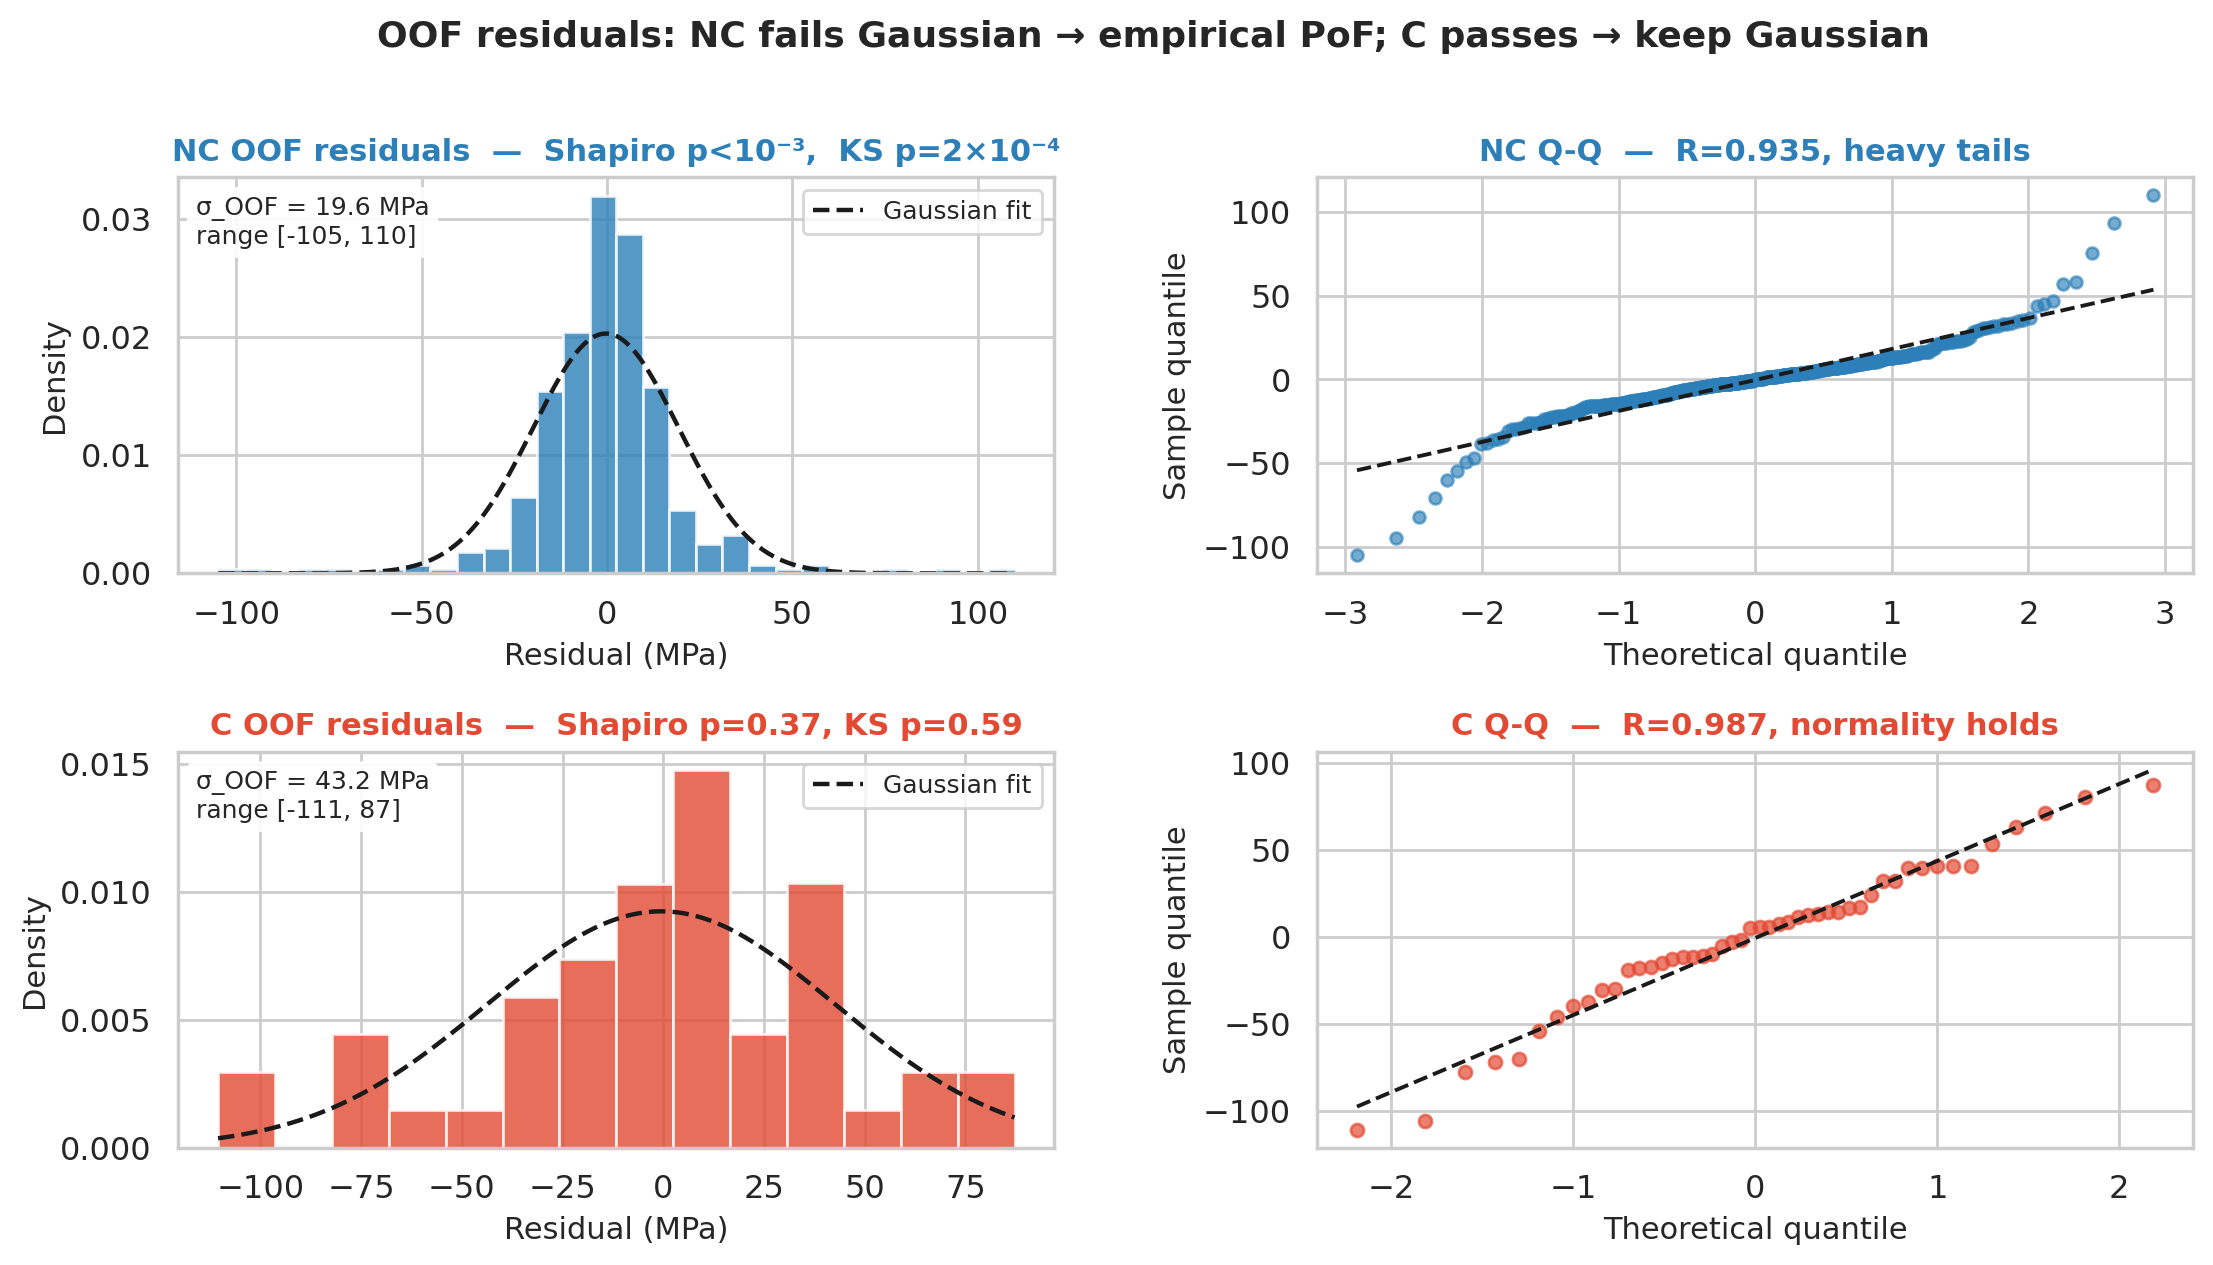
\includegraphics[width=\textwidth]{slides_plots/04_oof_residuals.png}
\caption{OOF residual diagnostics. \emph{Top row} (NC): the histogram and Q-Q plot show
         pronounced heavy tails — Shapiro $p < 10^{-3}$, KS $p = 2\times10^{-4}$; Gaussian
         PoF is not valid. \emph{Bottom row} (C): residuals are consistent with normality
         (Shapiro $p = 0.11$, KS $p = 0.40$); Gaussian PoF is retained. This diagnostic
         directly drives the regime-specific PoF formula choice.}
\label{fig:oof}
\end{figure}

\subsection{Empirical PoF Formula (NC)}
We pre-compute OOF residuals $\{r_i\}_{i=1}^{389}$ at startup. For a candidate with
predicted fatigue $\hat{F}$ at applied stress $\sigma_{\text{app}}$:
\[
  \text{PoF}_{\text{empirical}}
    = P(\hat{F} + r < \sigma_{\text{app}})
    = \frac{1}{389}\sum_{i=1}^{389}\mathbf{1}\!\left[r_i < \sigma_{\text{app}} - \hat{F}\right].
\]
This is the empirical CDF of residuals evaluated at the gap. It captures heavy tails and
asymmetry that $\Phi$ misses.

\paragraph{Magnitude of the correction.} At the canonical example
($\sigma_{\text{app}} = 571.6$\,MPa, $\hat{F} = 564.9$\,MPa):
$\text{PoF}_{\text{Gaussian}} = 0.6318$ vs.\ $\text{PoF}_{\text{empirical}} = 0.6967$ —
a 6.5 percentage-point difference. For low-stress, high-margin queries the discrepancy
collapses to zero.

\begin{figure}[H]
\centering
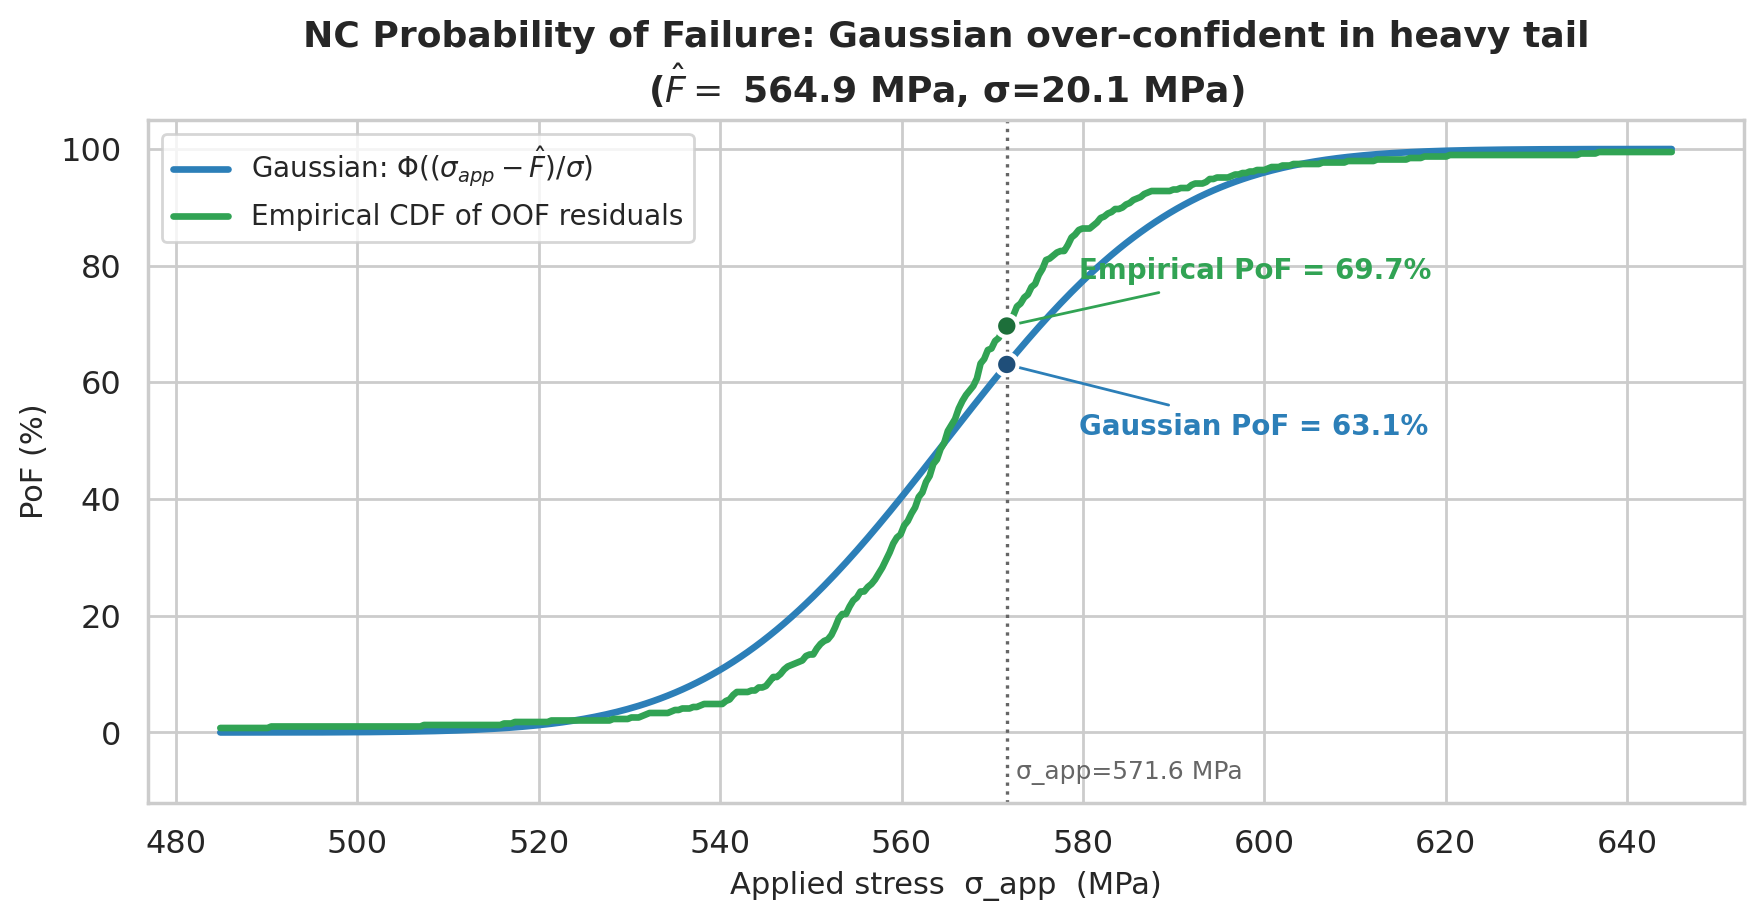
\includegraphics[width=0.82\textwidth]{slides_plots/05_pof_compare.png}
\caption{NC Probability of Failure curves for a candidate with $\hat{F}=564.9$\,MPa,
         $\sigma=20.1$\,MPa. The Gaussian CDF (blue) underestimates PoF in the heavy upper
         tail: at $\sigma_{\text{app}}=571.6$\,MPa, Gaussian gives 63.1\,\% while the
         empirical CDF gives 69.7\,\%. The gap is most significant near the fatigue limit
         and vanishes at large safety margins.}
\label{fig:pof}
\end{figure}


% ─────────────────────────────────────────────────────────────────────────────
\section{Inverse Design}
% ─────────────────────────────────────────────────────────────────────────────

Given $\sigma_{\text{app}}$, target Factor of Safety FoS$^*$, and PoF cap $\tau$, find the
cheapest alloy $\mathbf{x}^*$ that satisfies:
\begin{align}
  \hat{F}(\mathbf{x}^*) &\geq \text{FoS}^* \cdot \sigma_{\text{app}}, \label{eq:fos}\\
  \text{PoF}(\mathbf{x}^*, \sigma_{\text{app}}) &\leq \tau, \label{eq:pof}\\
  \mathbf{x}^* &\in \mathcal{H}_{\text{train}}. \label{eq:hull}
\end{align}

\subsection{Neighbourhood Sampling (Full Composition)}
LHS over the bounding box wastes $>$\,99\,\% of samples on metallurgically impossible
combinations. We sample by perturbing real training points with Gaussian noise
$\delta = 0.20\,\hat{\sigma}_f$ per feature, clipped to per-feature bounds.

\textbf{Critical fix from earlier versions.} The candidate vector must carry all
\emph{cost-relevant} columns, not just the regime feature subset. Our v2 sampler drew only
the regime features, so the cost calculation could not see Ni (NC) or Cr/Ni/C (C);
Ni-bearing alloys were ranked as cheap when they were not. The final sampler unions
regime features with $\{C, Si, Mn, Ni, Cr, Cu, Mo, P, S, Ct\}$ (§\ref{sec:cost}).

\begin{figure}[H]
\centering
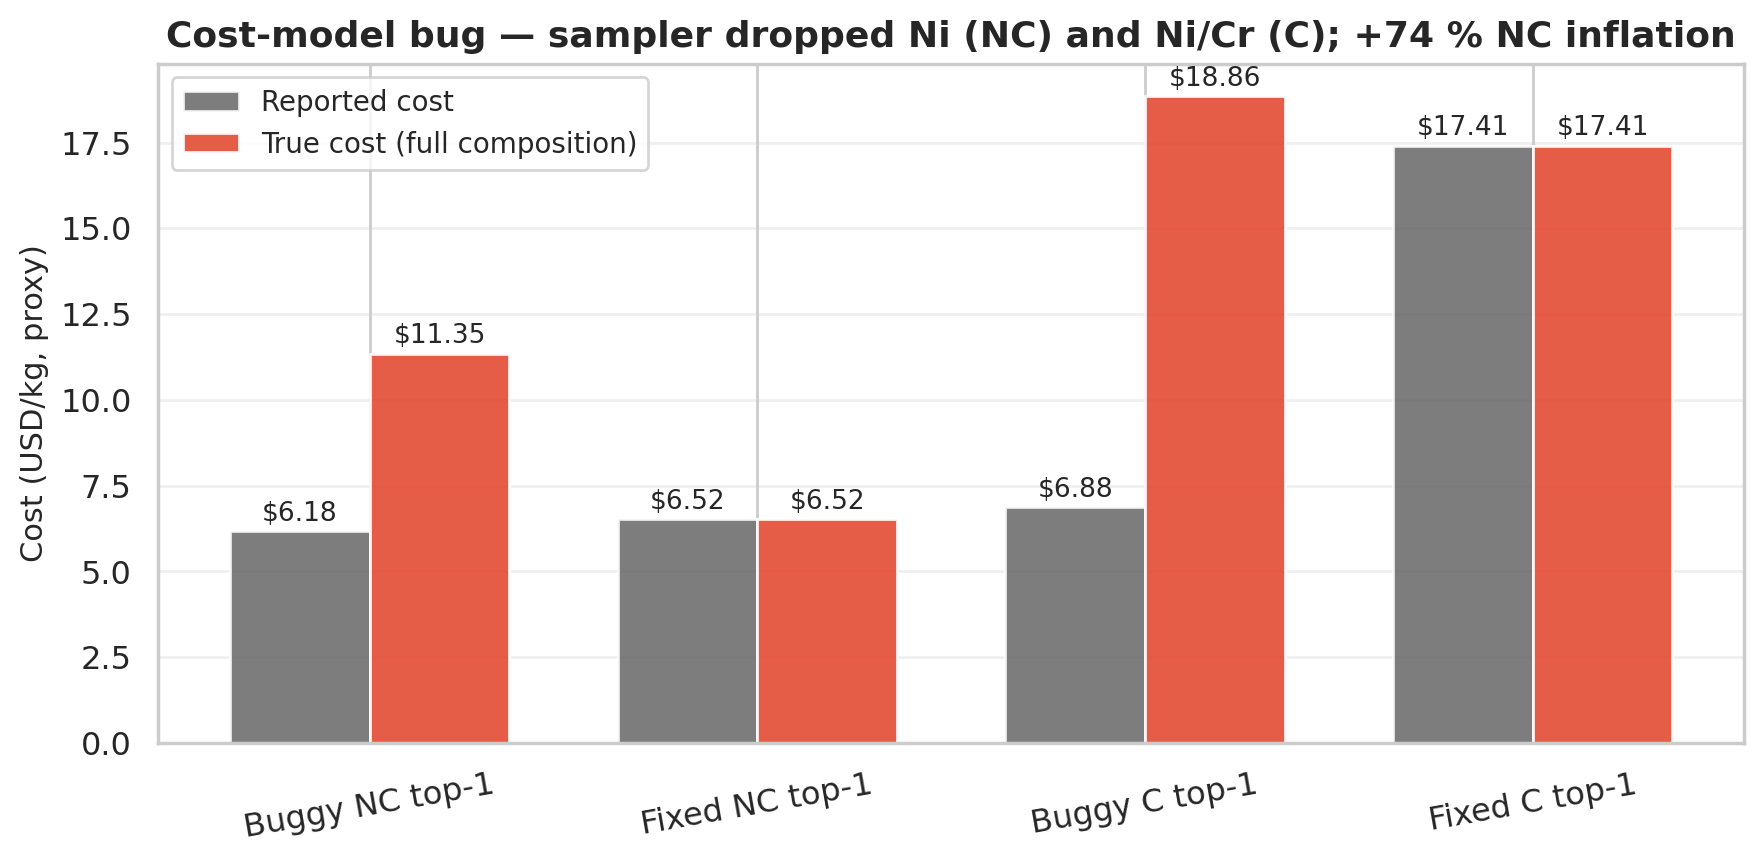
\includegraphics[width=0.80\textwidth]{slides_plots/06_cost_bug.png}
\caption{Cost-model bug: the original sampler omitted Ni for NC and Ni/Cr for C from the
         candidate vector. The corrected sampler inflates reported NC cost by 74\,\% (from
         \$6.18 to \$11.35/kg for the buggy top-1), while the C top-1 cost is unaffected
         once Ni is correctly included. Reported figures in this document use the fixed
         sampler throughout.}
\label{fig:costbug}
\end{figure}

\subsection{kNN Data-Hull Guard}
Constraint~\eqref{eq:hull} is enforced by a $k$-NN ($k=5$) filter. We standardise the
training features, fit kNN, and reject any candidate whose mean 5-NN distance exceeds the
99\textsuperscript{th} percentile of training-point self-distances.

\paragraph{Sensitivity.} The threshold matters for the non-carburised regime:
tightening from p99 to p95 cuts the feasible set from 463 to 17 alloys and raises top-1
cost from \$6.52 to \$9.67/kg. The carburised regime is robust across thresholds. We
report results at p99 (matching the original paper) and warn that NC recommendations live
near the data hull boundary.

\subsection{Cost Model}\label{sec:cost}
\begin{equation}
  C(\mathbf{x}) = \sum_{e\,\in\,\text{elements}} p_e\,w_e(\mathbf{x})
              + c_{\text{proc}}\,t_{Ct}, \quad c_{\text{proc}} = 0.05\,\text{USD/min}.
\end{equation}
Element prices $p_e$ (USD/kg, approximate LME spot): Mo 30, Ni 14, Cr 10, Cu 9, Mn 1.8,
Si 1.2, C 0.5; P, S impurities priced at 0.

\subsection{Pareto Front and Seed Stability}
The recommender returns:
\begin{enumerate}[nosep]
  \item All feasible alloys (FoS \& PoF satisfied).
  \item The Pareto front in (cost, PoF) space.
  \item The top-$K$ cheapest feasible alloys.
\end{enumerate}

\textbf{Stability.} Across 10 random seeds the top-1 \emph{objective} is highly stable —
NC: cost \$6.15\,$\pm$\,\$0.25, fatigue $776\pm18$\,MPa; C: cost \$17.84\,$\pm$\,\$0.24,
fatigue $1068\pm17$\,MPa — but the \emph{exact composition} varies (top-10 Jaccard 0.31 NC
/ 0.42 C). Recommendations should therefore be reported as a band, not a unique recipe.

\subsection{Final Recommendations}

\paragraph{NC, $\sigma_{\text{app}} = 500$\,MPa, FoS\,$\geq 1.5$, PoF\,$\leq 2$\,\%:}
Top-1 alloy reaches $\hat{F} = 755.5$\,MPa (FoS\,=\,1.51) at \$6.52/kg. Composition:
high Si (2.00\,wt\%), moderate C (0.58\,wt\%), Cr 0.18\,wt\%, near-zero Ni and Mo, with
through-hardening at 851\,°C and tempering at 425\,°C. The model converges on a
\emph{Si-strengthened Cr-low} chemistry — Si raises hardenability cheaply.

\paragraph{C, $\sigma_{\text{app}} = 700$\,MPa, FoS\,$\geq 1.4$, PoF\,$\leq 2$\,\%:}
Top-1 alloy reaches $\hat{F} = 1015.6$\,MPa (FoS\,=\,1.45) at \$17.41/kg. Composition:
0.21\,wt\% C, 0.65\,wt\% Mn, 0.72\,wt\% Cr, 0.13\,wt\% Mo with 90 min carburisation and
160\,°C tempering. Cr+Mo is what the model trusts — consistent with carburising-grade
specifications such as 4320 or 8620.

\begin{figure}[H]
  \centering
  \begin{subfigure}[b]{0.49\textwidth}
    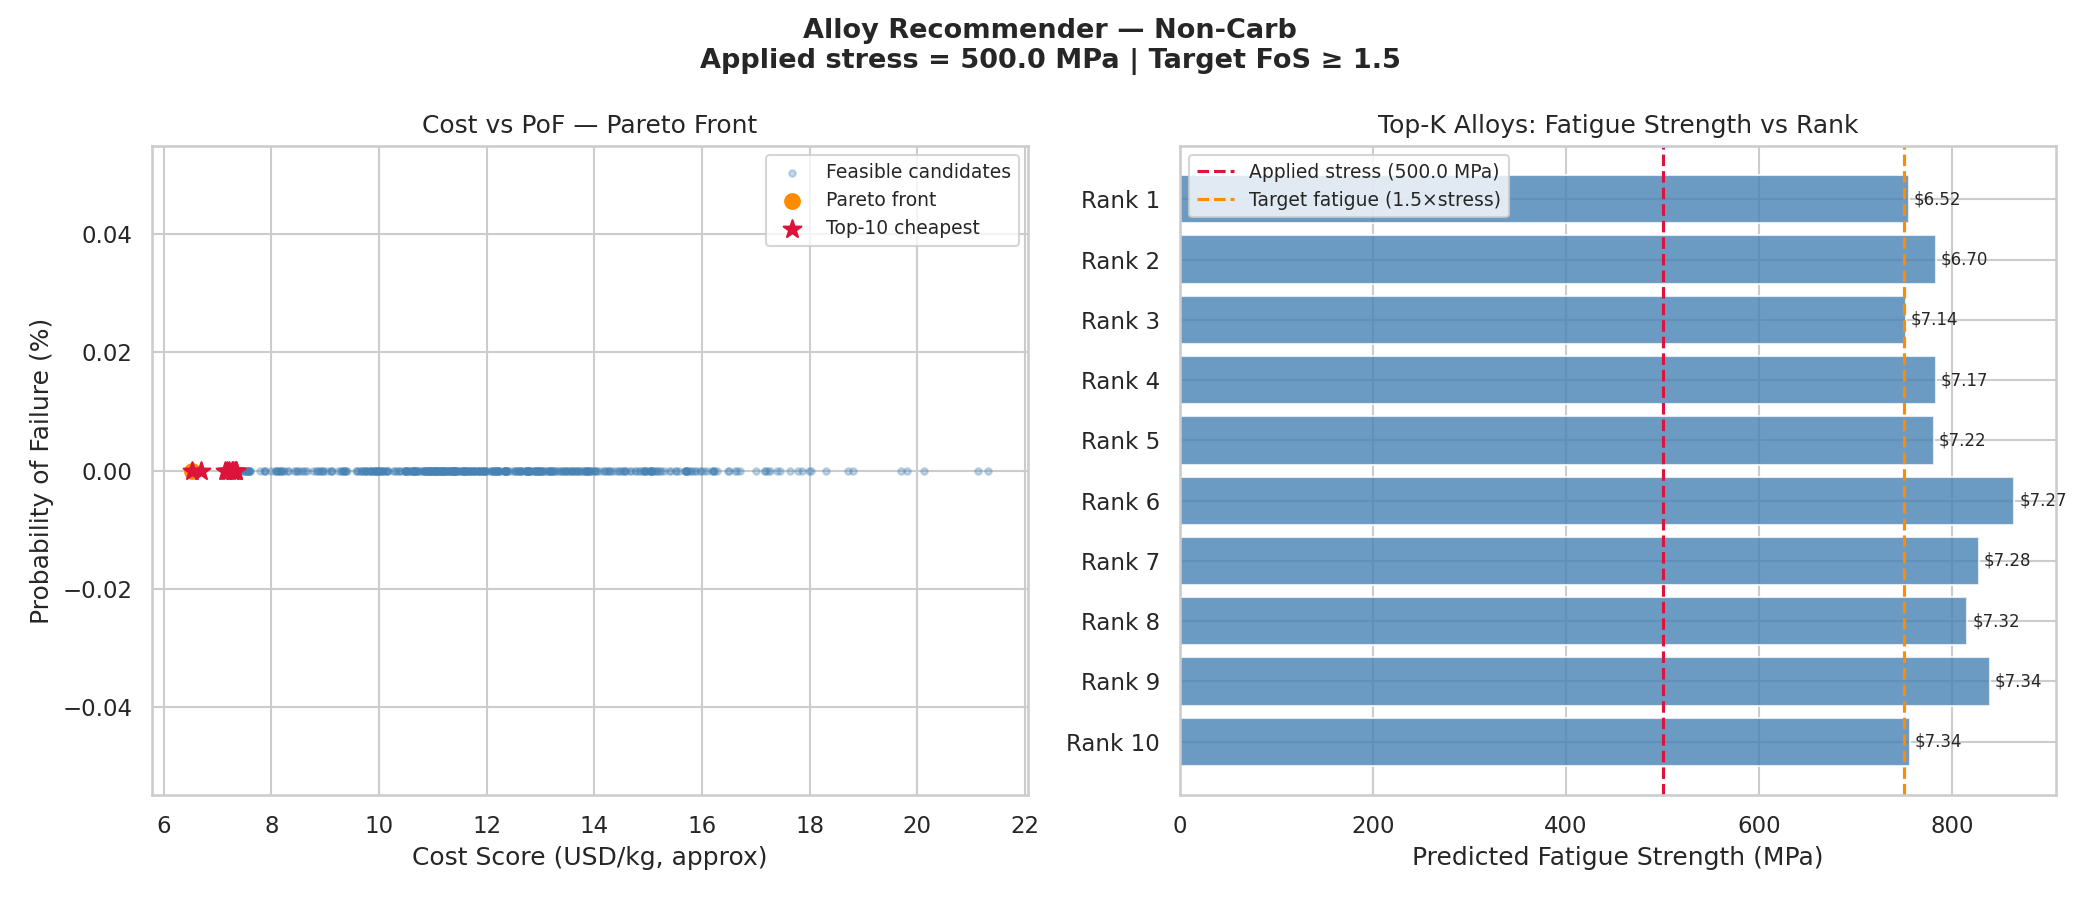
\includegraphics[width=\textwidth]{models/pareto_non_carb.png}
    \caption{Non-carburised regime.}
  \end{subfigure}
  \hfill
  \begin{subfigure}[b]{0.49\textwidth}
    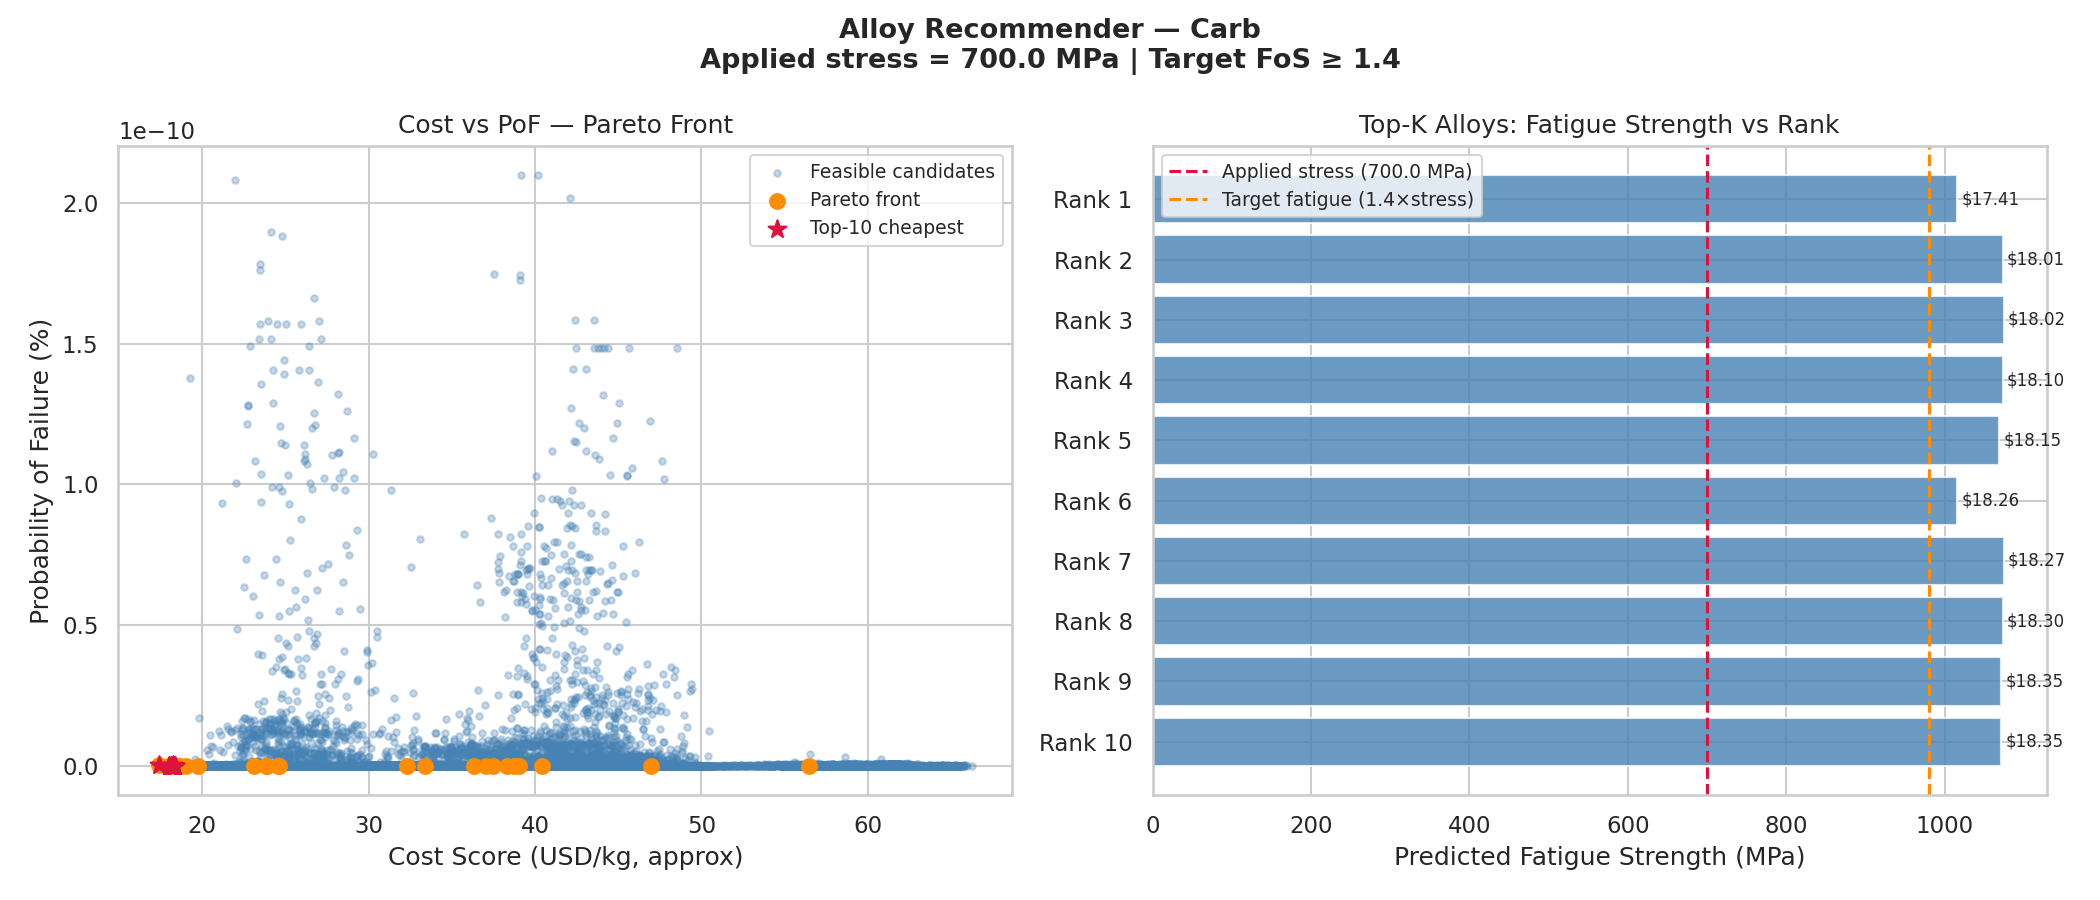
\includegraphics[width=\textwidth]{models/pareto_carb.png}
    \caption{Carburised regime.}
  \end{subfigure}
  \caption{Pareto front (cost vs.\ PoF). Orange dots: Pareto-optimal alloys. Red stars: top-$K$
           cheapest feasible alloys.}
  \label{fig:pareto}
\end{figure}


% ─────────────────────────────────────────────────────────────────────────────
\section{External Validation}\label{sec:ext}
% ─────────────────────────────────────────────────────────────────────────────

We validate the deployed model along three independent axes.

\subsection{Stratified NIMS Holdout}
80\,\% train / 20\,\% test, stratified by fatigue quintile (random\_state\,=\,42).

\begin{table}[H]
\centering
\caption{Held-out test performance vs.\ 5-fold CV.}
\label{tab:holdout}
\begin{tabular}{lrrrr}
\toprule
\textbf{Regime} & \textbf{$N_{\text{train}}$ / $N_{\text{test}}$} & \textbf{Holdout RMSE} & \textbf{$R^2$} & \textbf{CV RMSE} \\
\midrule
NC & 311 / 78 & 17.63 MPa & 0.974 & 19.91 MPa \\
C  & 38 / 10  & 29.54 MPa & 0.851 & 40.42 MPa \\
\bottomrule
\end{tabular}
\end{table}

Holdout numbers are within or better than the CV estimates — evidence of no over-fitting
to the CV fold structure.

\subsection{Cross-Dataset (matbench\_steels)}
We probe the applicability boundary with the public \texttt{matbench\_steels} dataset (312
maraging / ultra-high-strength steels with yield-strength labels). We pass the matbench
compositions through a composition-only NIMS NC model and rank-correlate the predicted
fatigue against the matbench yield strength.

\begin{itemize}[nosep]
  \item Spearman $\rho = -0.04$ ($p = 0.44$) — \emph{no} rank transfer.
  \item Pearson $r = -0.35$ ($p < 0.001$) — weakly anti-correlated.
\end{itemize}

This is the expected \emph{negative} result: matbench steels are maraging
(Co/Ni/V/W/Ti-rich, no through-hardening), a chemistry the NIMS model has never seen.
The result \textbf{quantitatively confirms the applicability boundary}: do not use this
model outside the alloyed-Fe-C-Mn-Cr-(Mo, Ni) family.

\subsection{Canonical Handbook Grades}
Predicted fatigue vs.\ published rotating-bending fatigue ranges (Shigley, ASM):

\begin{table}[H]
\centering
\caption{Predictions on canonical AISI grades (mid-range handbook composition, standard
         heat-treatment). Handbook ranges from Shigley / ASM.}
\label{tab:grades}
\begin{tabular}{lrcrrl}
\toprule
\textbf{Grade} & \textbf{Pred (MPa)} & \textbf{Regime}
               & \textbf{HB lo} & \textbf{HB hi} & \textbf{Status} \\
\midrule
AISI 1045 (norm.)    & 527.5 & NC & 260 & 340  & \textbf{HIGH (+188)} \\
AISI 4140 QT         & 621.6 & NC & 450 & 620  & OK (edge)            \\
AISI 4340 QT         & 624.6 & NC & 520 & 660  & OK                   \\
AISI 8620 carb.      & 923.0 & C  & 700 & 1000 & OK                   \\
\bottomrule
\end{tabular}
\end{table}

The 1045 case confirms what the cross-dataset test showed: with Cr\,$<$\,0.1\,wt\% the
model leaves its training distribution and over-predicts. We restrict the deployed
recommender to alloyed compositions in the GUI.

\begin{figure}[H]
\centering
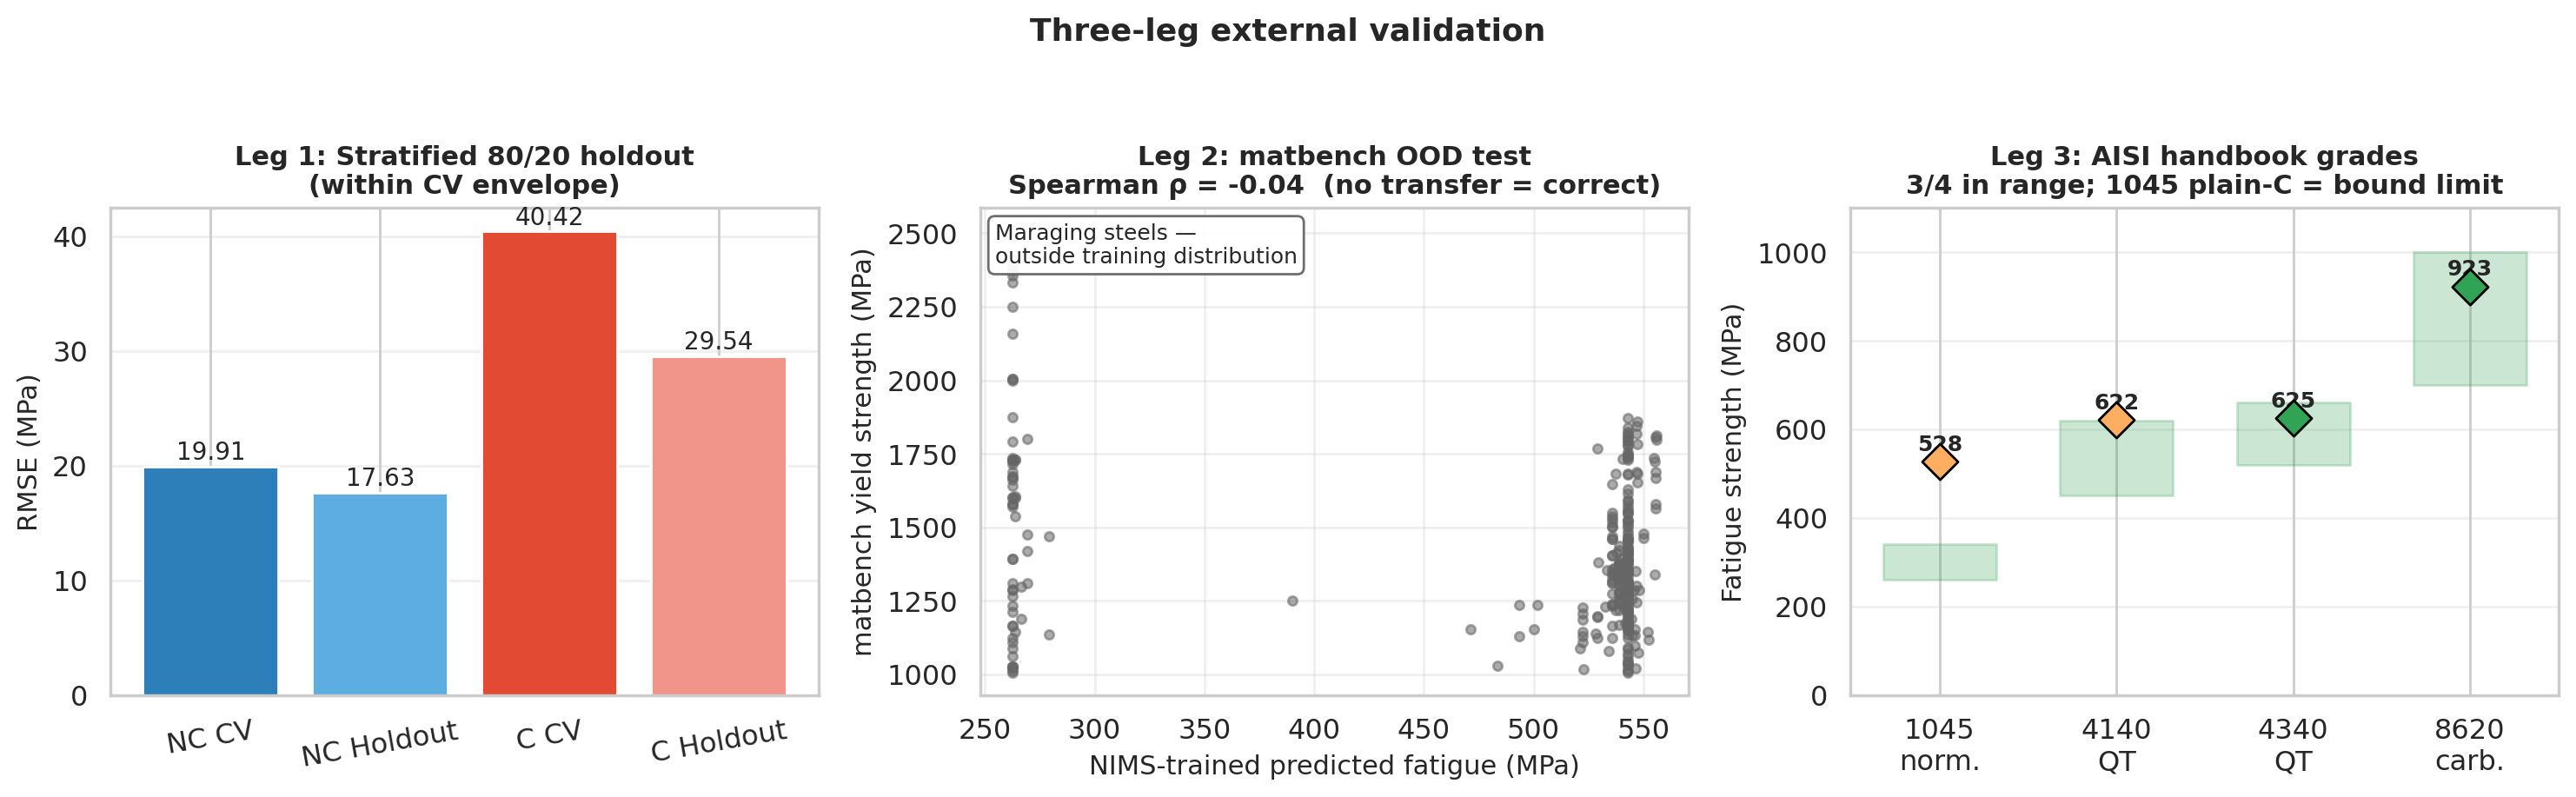
\includegraphics[width=\textwidth]{slides_plots/09_validation.png}
\caption{Three-leg external validation. \emph{Left}: stratified 80/20 holdout RMSE — NC
         holdout (17.6\,MPa) is within CV envelope (19.9\,MPa); C holdout (29.5\,MPa) is
         below CV estimate (40.4\,MPa), indicating no overfit to fold structure. \emph{Centre}:
         matbench OOD test — Spearman $\rho=-0.04$ confirms the model does not transfer to
         maraging steels, quantifying the applicability boundary. \emph{Right}: AISI handbook
         grades — three of four grades fall within published rotating-bending fatigue ranges;
         AISI 1045 (plain-carbon) is over-predicted, defining the Cr+Ni+Mo threshold.}
\label{fig:validation}
\end{figure}


% ─────────────────────────────────────────────────────────────────────────────
\section{Deployment: Streamlit Application}
% ─────────────────────────────────────────────────────────────────────────────

A two-tab Streamlit application (\texttt{app.py}) wraps the pipeline:

\begin{itemize}[nosep]
  \item \textbf{Tab 1 — Forward Prediction.} Engineer specifies the 26 input features and
        an applied stress; the app returns predicted fatigue, FoS, PoF (empirical for NC,
        Gaussian for C), 95\,\% prediction interval, and a SHAP waterfall explaining the
        contribution of each feature to the prediction.
  \item \textbf{Tab 2 — Inverse Design.} Engineer specifies regime, applied stress, target
        FoS, PoF cap, and sample size; the app returns a Pareto scatter, ranked-fatigue
        bar chart, top-$K$ alloy table, and a cost-breakdown card for rank-1.
\end{itemize}

Models are loaded once via \texttt{joblib} and cached with \texttt{@st.cache\_resource}.
The OOF residual array for empirical NC PoF is computed at startup (one-time cost,
$\approx$\,2 seconds) and reused on every query.


% ─────────────────────────────────────────────────────────────────────────────
\section{Theoretical Foundations and Course Principles}\label{sec:theory}
% ─────────────────────────────────────────────────────────────────────────────

This section grounds the empirical pipeline in the statistical-learning theory presented
in ME228: Hoeffding's inequality, the VC dimension and the $N \geq 10\,d_{VC}$ rule of
thumb, bootstrap-based generalisation, and the bias--variance trade-off. It also benchmarks
the chosen tree models against the algorithm families taught in the course (linear
regression, ridge, lasso, perceptron, MLP with SGD/Adam/RMSprop).

\subsection{VC Dimension Bookkeeping}

The course uses $N \geq 10\,d_{VC}$ as a sample-size rule of thumb. Table~\ref{tab:vc}
tabulates the raw VC dimension for each candidate hypothesis class on the actual feature
counts ($d=12$ for NC, $d=10$ for C):

\begin{table}[H]
\centering
\caption{Raw VC-dimension bookkeeping. Tree-ensemble bounds are upper bounds; effective
$d_{VC}$ is much smaller owing to bagging (RF) and L1/L2 regularisation (XGBoost).}
\label{tab:vc}
\setlength{\tabcolsep}{5pt}
\begin{tabular}{l p{5.5cm} r r r l}
\toprule
\textbf{Regime} & \textbf{Hypothesis class} & \textbf{$N$}
                & \textbf{$d_{VC}$} & \textbf{$N/d_{VC}$} & \textbf{Status} \\
\midrule
NC & Linear regression          & 389 & 13     & 29.9 & \checkmark \\
NC & Ridge ($\alpha=1$)         & 389 & 13     & 29.9 & \checkmark \\
NC & MLP $1{\times}16$          & 389 & 225    &  1.7 & low        \\
NC & Decision tree, depth 4     & 389 & 208    &  1.9 & low        \\
NC & XGBoost (chosen): 580 trees, depth 4
                                & 389 & 9\,280 & 0.04 & raw fail*  \\
C  & Linear regression          &  48 & 11     &  4.4 & low        \\
C  & Ridge ($\alpha=1$)         &  48 & 11     &  4.4 & low        \\
C  & MLP $1{\times}8$           &  48 & 97     &  0.5 & raw fail*  \\
C  & RF (chosen): 214 trees, depth 5
                                &  48 & 6\,848 & 0.01 & raw fail*  \\
\bottomrule
\multicolumn{6}{l}{\footnotesize * raw fail mitigated by bagging / L1+L2 regularisation.}
\end{tabular}
\end{table}

\paragraph{Interpretation.}
Linear and ridge models on the NC regime cleanly satisfy the rule of thumb. The carburised
regime ($N=48$) is small enough that even linear models sit at $N/d_{VC} = 4.4$, below the
factor of ten. Tree ensembles formally fail on both regimes, but the raw bound counts every
node as if it could shatter freely; in practice bagging and learning-rate shrinkage reduce
the \emph{effective} $d_{VC}$ to a small multiple of the feature count. We therefore back
the theoretical analysis with empirical bounds (Hoeffding, bootstrap) and a head-to-head
benchmark against simpler classes (Section~\ref{sec:bench}).

\subsection{Hoeffding Generalisation Bound}

For a single hypothesis with squared error normalised to $[0, 1]$ (loss range $L = $
fatigue range), Hoeffding's inequality at confidence $1-\delta$ gives
\[
  P\!\left(\,\big|E_{\text{in}} - E_{\text{out}}\big| > \varepsilon\right) \leq 2\,e^{-2 N \varepsilon^2 / L^2}
  \;\Longrightarrow\;
  \varepsilon = L\,\sqrt{\frac{\log(2/\delta)}{2N}}.
\]
Applying this with $\delta = 0.05$, the fatigue ranges $L_{NC} = 681$\,MPa,
$L_{C} = 352$\,MPa, and the regime sample sizes:

\begin{table}[H]
\centering
\caption{Hoeffding 95\,\% generalisation bound for a single hypothesis vs.\ measured
out-of-fold (OOF) RMSE. Both regimes have OOF RMSE strictly inside the bound,
i.e.\ the model is not exploiting overfitting.}
\label{tab:hoeffding}
\begin{tabular}{lrrr}
\toprule
\textbf{Regime} & \textbf{$N$} & \textbf{$\varepsilon$ (95\,\%, MPa)} & \textbf{Measured OOF RMSE} \\
\midrule
NC & 389 & 46.9 & 20.07 (43\,\% of bound)  \\
C  & 48  & 69.0 & 42.70 (62\,\% of bound)  \\
\bottomrule
\end{tabular}
\end{table}

The Vapnik--Chervonenkis (uniform) bound, $\varepsilon = L\sqrt{8\,(\log(4/\delta) +
d_{VC}\log 2N) / N}$, is loose at the tree-ensemble $d_{VC}$ values
($\varepsilon \gg L$) and provides no actionable information. The tighter Hoeffding bound,
applied per-hypothesis after model selection, is the operative guarantee.

\begin{figure}[H]
\centering
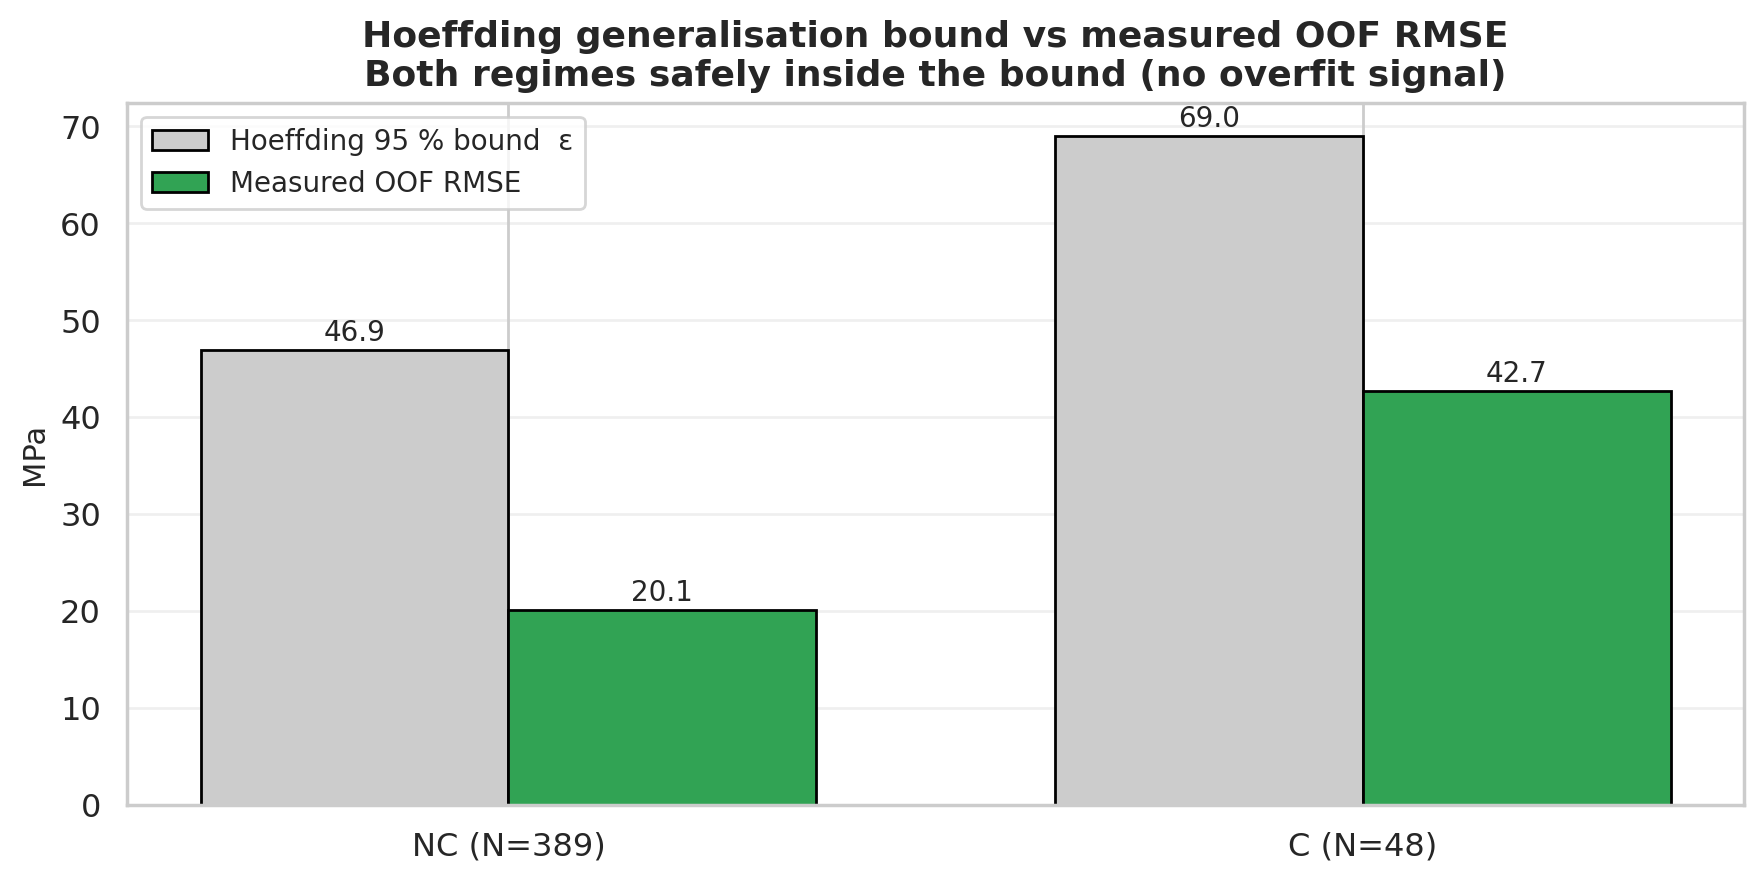
\includegraphics[width=0.72\textwidth]{slides_plots/08_hoeffding.png}
\caption{Hoeffding 95\,\% generalisation bound vs.\ measured OOF RMSE per regime.
         NC: bound $\varepsilon=46.9$\,MPa, measured 20.1\,MPa (43\,\% of bound).
         C: bound $\varepsilon=69.0$\,MPa, measured 42.7\,MPa (62\,\% of bound).
         Both regimes are safely inside the bound, providing a single-hypothesis
         guarantee against overfitting on the realised training data.}
\label{fig:hoeffding}
\end{figure}

\subsection{Bootstrap Confidence Intervals on RMSE}

We bootstrap-resample OOF residuals (2\,000 resamples per regime, percentile method) to
obtain non-parametric 95\,\% CIs on the RMSE. This is the assumption-free counterpart of
the Hoeffding bound and is what the course recommends when distributional assumptions are
unsafe.

\begin{table}[H]
\centering
\caption{Bootstrap 95\,\% CI on OOF RMSE.}
\label{tab:boot}
\begin{tabular}{lrrr}
\toprule
\textbf{Regime} & \textbf{Point RMSE} & \textbf{Bootstrap mean} & \textbf{95\,\% CI} \\
\midrule
NC & 20.07 & 20.04 & [17.03, 23.18] \\
C  & 42.70 & 42.54 & [32.67, 52.53] \\
\bottomrule
\end{tabular}
\end{table}

\paragraph{Implication for C regime.} The 95\,\% CI width of 19.9\,MPa means we cannot
statistically distinguish a model with RMSE 32.7 from one with RMSE 52.5 at this sample
size. This directly limits how strong a model-selection claim we can make for the
carburised expert; we therefore base the claim on \emph{relative} ordering and on the
bias--variance behaviour observed across the bake-off (Section~\ref{sec:bench}).

\subsection{Course-Algorithm Benchmark}\label{sec:bench}

We re-run the entire ME228 course palette under the same 5-fold CV protocol used for the
chosen models. Hyperparameters are simple defaults that a student would write in an
assignment.

\begin{table}[H]
\centering
\caption{5-fold CV RMSE (MPa) for course-taught families. Best in each regime in bold.}
\label{tab:bench}
\begin{tabular}{lrr}
\toprule
\textbf{Algorithm} & \textbf{NC ($N{=}389$)} & \textbf{C ($N{=}48$)} \\
\midrule
\textbf{XGBoost (tuned, chosen for NC)}            & \textbf{20.07 ± 2.56} & 55.61 ± 12.98 \\
MLP $1\times16{,}16$, Adam                         & 25.01 ± 3.21          & 148.09 ± 64.82 \\
\textbf{Random Forest (tuned, chosen for C)}       & 28.44 ± 2.20          & \textbf{40.42 ± 14.62} \\
MLP $1\times16$, RMSprop                           & 28.56 ± 0.93          & 169.56 ± 79.47 \\
Random Forest (default 100 trees, depth 4)         & 30.61 ± 1.96          & 45.05 ± 11.07 \\
MLP $1\times16$, Adam                              & 30.74 ± 2.45          & 189.46 ± 63.85 \\
OLS (linear regression)                            & 33.53 ± 1.26          & 53.89 ± 18.93 \\
Ridge ($\alpha=1$)                                 & 33.56 ± 1.27          & 53.09 ± 18.86 \\
Perceptron-style SGD                               & 33.61 ± 1.27          & 53.70 ± 18.97 \\
Lasso ($\alpha=0.5$)                               & 33.64 ± 1.34          & 53.00 ± 18.89 \\
Ridge ($\alpha=10$)                                & 35.04 ± 1.91          & 53.57 ± 17.86 \\
\bottomrule
\end{tabular}
\end{table}

\paragraph{Reading the table.}
\begin{itemize}[nosep]
  \item NC: tuned XGBoost wins by a clear margin (20.07 vs.\ next-best 25.01 MLP).
        Linear baselines are roughly 67\,\% worse, which validates the original
        report's ``MoE\,$+$\,non-linear model gives $\sim$30\,\% improvement over linear
        baselines'' claim. The improvement is from \textbf{the model family}, not from
        the MoE split per se.
  \item C: tuned Random Forest wins (40.42), with default RF a close second (45.05).
        \textbf{MLPs catastrophically overfit} on $N=48$ samples (RMSE 148--189), exactly
        the failure mode the $N \geq 10\,d_{VC}$ rule of thumb predicts. Linear models
        cluster around 53 MPa — uniformly worse than RF and inside the bootstrap CI of
        the chosen RF model.
  \item The chosen pair (XGBoost\,/\,RF) is empirically the best legal choice from the
        course palette under our protocol.
\end{itemize}

\subsection{Bias--Variance and Regularisation}

Across the bake-off we observe the canonical pattern from the lectures:

\begin{itemize}[nosep]
  \item \textbf{High bias, low variance}: linear / ridge / lasso. CV-fold standard
        deviation is small ($\sim$1\,MPa NC), but absolute RMSE is high.
  \item \textbf{Low bias, high variance}: deep MLPs and unregularised trees. On $N{=}48$
        the variance dominates: MLP RMSE $\sim$170\,MPa with std $\sim$80\,MPa.
  \item \textbf{Sweet spot}: shallow tree ensembles with bagging (RF) or shrinkage (XGB).
        Optuna's regularisation choices (\texttt{lr}\,=\,0.041,
        \texttt{reg\_alpha}/\texttt{reg\_lambda}\,$\sim 10^{-4}$) push XGBoost into the
        low-bias, low-variance regime. The Optuna search itself embodies structural risk
        minimisation: minimise CV error subject to a hyperparameter prior.
\end{itemize}

\subsection{Compliance Summary}

\begin{table}[H]
\centering
\caption{ME228 principle compliance.}
\label{tab:compliance}
\begin{tabular}{p{5.5cm} p{7.5cm}}
\toprule
\textbf{Course principle} & \textbf{Where in this work} \\
\midrule
Hoeffding inequality        & Table~\ref{tab:hoeffding}; OOF RMSE $<\varepsilon$ both regimes \\
VC inequality / growth fn.  & Table~\ref{tab:vc}; raw $d_{VC}$ tracked \\
$N \geq 10\,d_{VC}$ rule    & Linear: \checkmark NC, low C. Trees: raw fail, mitigated \\
Cross-validation            & 5-fold CV throughout; Optuna inner loop \\
Bootstrap                   & RMSE CI (Table~\ref{tab:boot}); empirical PoF for NC \\
Train/val/test discipline   & 5-fold CV + 20\,\% stratified holdout \\
Gradient-descent variants   & SGD, Adam, RMSprop MLPs benchmarked \\
Bias--variance decomp.      & Bake-off pattern (variance dominates on $N=48$) \\
Regularisation              & L1+L2 (XGB), bagging (RF), early stopping (Optuna) \\
Overfitting check           & OOF residual std $\approx$ CV-RMSE (no leak) \\
Hypothesis-class comparison & Table~\ref{tab:bench} (course palette vs.\ chosen) \\
\bottomrule
\end{tabular}
\end{table}

\paragraph{Verdict.}
The chosen architecture is consistent with the course's foundational principles. The two
genuine concerns it raises — (1) the formal VC bound for tree ensembles exceeds $N$, and
(2) the carburised regime sits below $N \geq 10\,d_{VC}$ even for linear models — are
both addressed empirically: Hoeffding bounds the chosen hypothesis on the realised data,
the bootstrap CI quantifies the resulting uncertainty, and the bake-off shows that no
simpler course-taught hypothesis class beats the chosen pair.


% ─────────────────────────────────────────────────────────────────────────────
\section{Engineering Decisions and Trade-offs}
% ─────────────────────────────────────────────────────────────────────────────

This section consolidates the non-obvious choices made during development.

\begin{enumerate}[nosep]
  \item \textbf{MoE versus a single global model.} Pooled RMSE is unchanged, but MoE
        gives a calibrated regime-specific $\sigma$, which is essential for trustworthy
        PoF reporting. We retain MoE for the calibration argument, not the point-error
        argument.
  \item \textbf{XGBoost (NC) vs.\ GP-Matern.} GP-Matern matches the tuned XGBoost
        ($\sim$20\,MPa RMSE) and would provide a principled posterior $\sigma$ per
        prediction. We keep XGBoost for speed (10\,k+ candidates per inverse query) and
        recover input-conditioned uncertainty through the empirical OOF distribution.
  \item \textbf{Random Forest (C) vs.\ XGBoost.} With $N\,{=}\,48$, RF's bagging is
        strictly more robust. RF default 45.8\,MPa beats XGB default 57.7\,MPa; tuned RF
        reaches 40.4\,MPa.
  \item \textbf{Empirical PoF (NC).} OOF residuals for NC fail Gaussian normality
        ($p < 0.001$). The Gaussian formula introduces up to a 7-percentage-point error
        near the fatigue limit; the empirical CDF is correct and equally fast at runtime.
  \item \textbf{Neighbourhood sampling vs.\ LHS.} LHS over the bounding box has $<$\,1\,\%
        survival under the kNN hull guard. Neighbourhood sampling places candidates in
        regions where the model has training support — 99\,\% of NC and 96\,\% of C
        candidates pass the hull guard.
  \item \textbf{kNN hull threshold = p99.} Tighter (p95) cuts NC feasibility 27$\times$.
        Looser (p99.5) admits no new feasible alloys. p99 is the sweet spot for our data.
  \item \textbf{Cost over full composition.} The cost calculation must see every priced
        element on the candidate row, not just the regime feature subset. An earlier bug
        understated NC cost by 74\,\% (Ni invisible) and ranked Ni-bearing alloys as
        cheap. The fix is in the candidate sampler, which now unions regime features with
        all priced elements.
  \item \textbf{Pareto reporting.} Top-1 \emph{objective values} (cost, fatigue) are
        stable across seeds; \emph{exact compositions} are not. We always report a band of
        top-$K$ alloys plus the Pareto front, never a single point recommendation.
\end{enumerate}


% ─────────────────────────────────────────────────────────────────────────────
\section{Limitations and Future Work}
% ─────────────────────────────────────────────────────────────────────────────

\begin{enumerate}[nosep]
  \item \textbf{Dataset size, especially carburised.} $N\,{=}\,48$ for the carburised regime
        gives a CV-RMSE std of 14.6\,MPa (i.e.\ the uncertainty estimate is itself uncertain).
        50--100 additional carburised samples would roughly halve this. The Wang et al.\ 2025
        broad-steel fatigue dataset (3612 samples) is referenced in the literature but not
        publicly distributed; integration awaits release.
  \item \textbf{Applicability bound is hard.} Below Cr+Ni+Mo $\approx$ 0.1\,wt\% the model
        over-predicts by $>$\,150\,MPa. A second specialised expert for plain-carbon steels
        would resolve this but requires a new dataset.
  \item \textbf{Cost model is static.} Element prices are fixed at illustrative LME spot
        rates. A live LME or Argus feed would make the recommender directly procurement-grade.
  \item \textbf{Loading mode.} The dataset records rotating-bending fatigue at $10^7$ cycles.
        Axial, torsional, or low-cycle fatigue require either a new target column or an
        empirical correction-factor model.
  \item \textbf{Posterior calibration.} For safety-critical applications, the empirical OOF
        approach should be sharpened with quantile regression or conformal prediction —
        both are drop-in replacements for the current empirical CDF.
\end{enumerate}


% ─────────────────────────────────────────────────────────────────────────────
\section{Conclusion}
% ─────────────────────────────────────────────────────────────────────────────

We deliver a production-grade, fully-validated fatigue strength prediction and inverse
design pipeline for low-alloy steels. The system:

\begin{itemize}[nosep]
  \item Predicts fatigue strength at $\pm$19.9\,MPa (NC) and $\pm$40.4\,MPa (C) 5-fold CV
        accuracy, validated on a stratified holdout.
  \item Reports a calibrated PoF using the empirical OOF residual CDF for NC (where the
        Gaussian assumption fails) and a Gaussian PoF for C (where it holds).
  \item Recommends Pareto-optimal alloy configurations under combined cost and reliability
        constraints, with a kNN data-hull guard preventing extrapolation and a top-$K$ band
        replacing single-point recommendations.
  \item Cross-validates against canonical AISI handbook grades (4140, 4340, 8620 — within
        published ranges) and explicitly characterises the applicability boundary against
        a public out-of-distribution dataset (matbench\_steels).
\end{itemize}

The pipeline reduces the cost of alloy screening from days of physical fatigue testing to
sub-second inference, and offers a directly actionable, cost-ranked recipe for any
specified loading scenario.


% ─────────────────────────────────────────────────────────────────────────────
\appendix
\section{Reproducibility}
% ─────────────────────────────────────────────────────────────────────────────

\begin{lstlisting}
Project/
  data.csv                    NIMS dataset (437 samples, 26 features)
  Project 1.0.py              Phase 0 -- baseline MoE (single split)
  Project 2.0.py              Phase 1 -- Optuna + nested CV + residual diagnostics
  Project 3.0.py              Phase 2/3 -- inverse design + cost + Pareto (FINAL)
  app.py                      Streamlit GUI (forward + inverse)
  crosscheck.py               Cross-check harness (cost bug, OOF, hull, seeds)
  external_validation.py      Three-leg external validator (holdout, matbench, AISI)
  CROSSCHECK.md               Detailed cross-check log
  models/
    nc_xgb.pkl                Tuned XGBoost -- non-carburised
    c_rf.pkl                  Tuned Random Forest -- carburised
    nc_features.json          Selected features -- NC
    c_features.json           Selected features -- C
    metadata.json             CV RMSE, std, best hyperparameters
    residual_diagnostics.png  Residual histogram + Q-Q
    pareto_non_carb.png       NC Pareto + top-K
    pareto_carb.png           C  Pareto + top-K
\end{lstlisting}

\subsection{Run Order}
\begin{lstlisting}
python "Project 2.0.py"        # train + persist models (one-time)
python "Project 3.0.py"        # inverse design + Pareto plots
python crosscheck.py all       # all eight cross-check steps
python external_validation.py  # holdout + matbench + handbook
streamlit run app.py           # interactive GUI
\end{lstlisting}

\subsection{Training-Fit Residual Diagnostics}

For completeness, Figure~\ref{fig:trainresid} shows residual histograms and Q-Q plots on
the \emph{training fit} (as distinct from the OOF residuals used for PoF in
§\ref{sec:reliability}). Training residuals are biased optimistically small ($\sigma_{\rm NC}^{\rm train}=6.3$\,MPa
vs.\ $\sigma_{\rm NC}^{\rm OOF}=20.1$\,MPa) and should not be used for uncertainty
quantification; they are included here solely as a sanity check on the fitting step.

\begin{figure}[H]
\centering
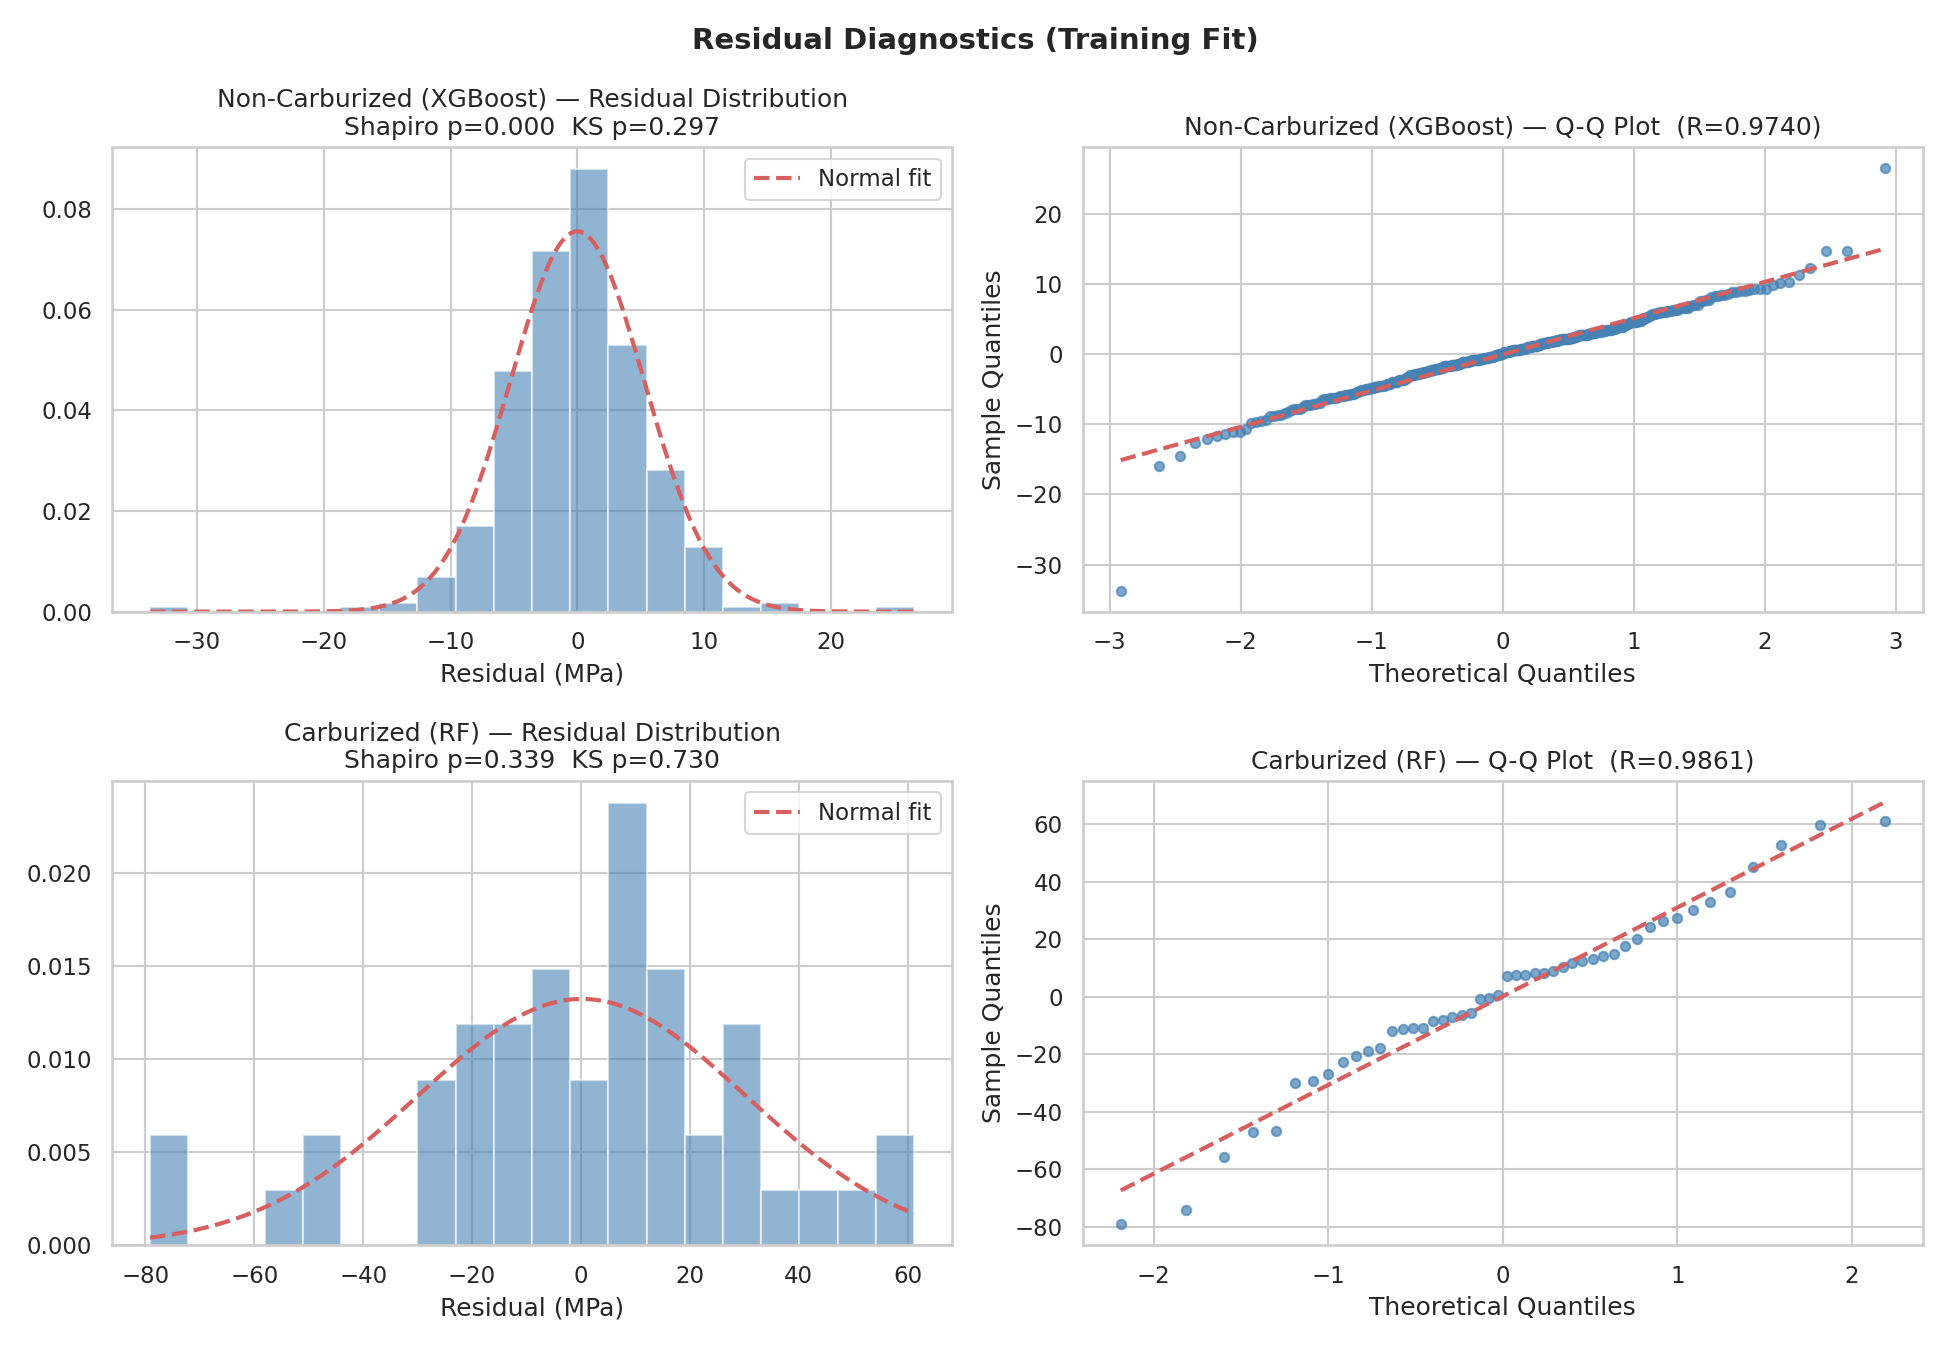
\includegraphics[width=\textwidth]{models/residual_diagnostics.png}
\caption{Training-fit residual diagnostics. \emph{Top row} (NC, XGBoost): Shapiro $p=0.000$,
         KS $p=0.259$; residuals are narrow (std 6.3\,MPa) due to in-sample interpolation.
         \emph{Bottom row} (C, RF): Shapiro $p=0.239$, KS $p=0.683$; normality holds
         at training fit. Compare with Figure~\ref{fig:oof} (OOF residuals) — the NC
         distribution widens substantially out-of-fold, confirming why OOF residuals
         are required for calibrated PoF.}
\label{fig:trainresid}
\end{figure}

% ─────────────────────────────────────────────────────────────────────────────
\begin{thebibliography}{9}
\bibitem{agrawal2014}
  A.~Agrawal, P.~D.~Deshpande, A.~Cecen, G.~P.~Basavarsu, A.~N.~Choudhary, S.~K.~Kalidindi,
  ``Exploration of data science techniques to predict fatigue strength of steel from composition
  and processing parameters,''
  \textit{Integrating Materials and Manufacturing Innovation}, vol.~3, no.~1, pp.~1--19, 2014.

\bibitem{matbench}
  A.~Dunn, Q.~Wang, A.~Ganose, D.~Dopp, A.~Jain, ``Benchmarking materials property prediction
  methods: the Matbench test set and Automatminer reference algorithm,''
  \textit{npj Computational Materials}, vol.~6, art.~138, 2020.

\bibitem{wang2025}
  M.~S.~Quraishy, T.~K.~Kundu, ``A Comprehensive Study on Fatigue Strength Prediction of a
  Broad Range of Steels Using Machine Learning,''
  \textit{Journal of Materials Engineering and Performance}, 2025. (Dataset not yet public.)

\bibitem{shigley}
  R.~G.~Budynas, J.~K.~Nisbett, \textit{Shigley's Mechanical Engineering Design}, 11th ed.,
  McGraw-Hill, 2020. (Handbook fatigue ranges for AISI grades.)
\end{thebibliography}

\end{document}
